\documentclass{NLE}

\usepackage{times,verbatim} % Please do not comment this
\usepackage{graphicx}
%\input{psfig.sty}

\usepackage{color,soul}
\usepackage[linesnumbered,ruled]{algorithm2e}
\usepackage{courier}
\usepackage{lmodern}
\usepackage{tcolorbox}
\usepackage{url}
\usepackage{enumitem}

\title{A compression based toolkit for text processing}
\author{W.\ns J.\ns T\ls E\ls A\ls H\ls A\ls N\ls}
%     School of Computer Science, Bangor University\\
%	Dean Street, Bangor, Gwynedd LL57 1UT, UK\\
%	email: w.j.teahan@bangor.ac.uk}

\shorttitle{A compression based toolkit for text processing}

\begin{document}

\maketitle

\begin{abstract}

A novel compression-based toolkit for modelling and processing sequential text is described. The design of the toolkit adopts 
an encoding perspective---applications are considered to be problems in searching for the best encoding of different transformations of the source text into the target text. The paper describes a two phase `noiseless channel model' architecture that underpins the toolkit which models the text processing as a lossless communication down a noise-free channel.
The transformation and encoding that is performed in the first phase must be both lossless and reversible. The role of the verification and decoding second phase is to verify the correctness of the communication of the target text that is produced by the application. The paper also argues that this encoding based approach has several advantages over the decoding based approach of the standard noisy channel model.

The paper describes the toolkit's libraries whose purpose are intended to shield the user from details of the modelling and probability estimation process in order to enable different implementations of models to be replaced transparently in application programs. 
The design behind the toolkit is probabilistic: that is, it supplies the probability of the next symbol in the sequence. It is general enough to deal accurately with Markov-based models that include escapes for probabilities. The concepts abstracted by the toolkit's design are explained together with details of the library calls. The pseudo-code  for a number of algorithms are also described for the applications that the toolkit implements including encoding, decoding, classification, model building, parallel sentence alignment, word segmentation and language segmentation. Some implementation details, memory usage and execution speeds are also discussed for these applications.


\end{abstract}

\section{Introduction}

This paper describes the design and implementation of a compression based toolkit for text processing.
The toolkit can be applied to any type of text since it involves the application of text compression algorithms designed for general
text. However, this paper will focus specifically on its application to natural language processing (NLP) and the processing of written text.

The toolkit is based on an earlier Application Programming Interface (API) designed by Cleary \& Teahan~\shortcite{cle97} for modelling sequential text using text compression models. The purpose of the toolkit is to simplify the design of applications where textual models are needed such as text compression, categorisation, and segmentation, by shielding the user from the details of the modelling and estimation process. Another purpose is to enable different implementations of models to be replaced transparently in application programs.  
The design behind the toolkit is probabilistic: that is, it supplies the probability of the next symbol in the sequence. It is general enough to deal accurately with Markov-based models that include escapes for probabilities such as the Prediction by Partial Mapping (PPM) text
compression scheme~\cite{cle84,mof90}.

During the development of the API and earlier versions of the toolkit, it became apparent that broadening its scope to encompass a much wider range of text operations was possible. It was found that many of the API-based programs that were devised had remarkable similarities in the underlying source code---despite the programs being complex, only a few changes were needed to define the key differences between the applications~\cite{mah08}. These observations have led to the creation of the Tawa\footnote{Tawa is a common broadleaf tree found in New Zealand. The acronym stands for {\bf T}ext {\bf A}nalyser from {\bf Wa}ikato since it was first developed at Waikato University, and subsequently improved over two decades at Lund, Robert Gordon and Bangor Universities.} Toolkit described in this paper. The toolkit is now available for download\footnote{\url{http://aiia.cs.bangor.ac.uk/software/Tawa-1.0.tgz}} and is a comprehensive extension of the original Cleary \& Teahan API and an updated version of the TMT toolkit~\cite{mah08} that was based on the API. The toolkit provides a powerful method for classifying, mining and transforming text. The purpose of this paper is to describe the design and implementation behind the toolkit including its architecture, libraries, and sample applications.

The contributions of this paper are as follows:

\begin{itemize}
\item The compression-based architecture which underpins the toolkit, and how it differs from the standard architecture for NLP, the noisy channel model, is fully described for the first time.
The paper explains the encoding approach taken by the toolkit's architecture as opposed to the decoding approach of the noisy channel model and how it provides a wider range of processing possibilities.
\item This paper is the first to discuss in detail the toolkit's libraries, including the methods and objects used.
The toolkit provides an extensive update of previous versions including an overhaul of the transformation libraries that simplifies
and consolidates the processes previously used.
\item The algorithms behind each of the toolkit's main applications are also described for the first time.
\end{itemize}

The paper is organised as follows. In the next section, we detail the design of the toolkit and its underlying architecture. The toolkit's libraries are then described followed by pseudo-code for some sample applications built using the libraries. A list of specific applications
implemented by the toolkit, sample use, implementation details, memory usage and execution speeds and search algorithms are discussed in Section~\ref{section.samples}. The paper then discusses previously published experimental results, and related work and provides a conclusion and discussion of future work in the final section.

\section{The toolkit's design}
\label{section.design}

In this section, the overall design of the Tawa toolkit shown diagrammatically in Figure~\ref{figure:overall-design} is described. The aim of the toolkit is to simplify the conceptualisation and implementation for a broad range of text mining and NLP applications involving textual transformations. The toolkit presently consists of nine main applications (such as {\bf align}, {\bf classify}, {\bf codelength}, and so on). These applications are built using three libraries---\verb|TXT| for text-based operations, \verb|TLM| for language modelling operations, and \verb|TTM| for transformation operations. These libraries are detailed in Section~\ref{section.libraries} and sample methods discussed in Section~\ref{section.methods}. Nine applications that demonstrate how the libraries work are detailed in Section~\ref{section.samples}. These applications provide useful tools for many NLP operations that have often produced state-of-the-art results as detailed in Section~\ref{section.results}. Underlying the design of these libraries and applications is a novel compression-based architecture called the ``Noiseless Channel Model'' to distinguish it from the standard ``Noisy Channel Model''. The key insight is that each application performs a search to find the best encoding of the target message rather than performing a decoding of the observed message.

\begin{figure}
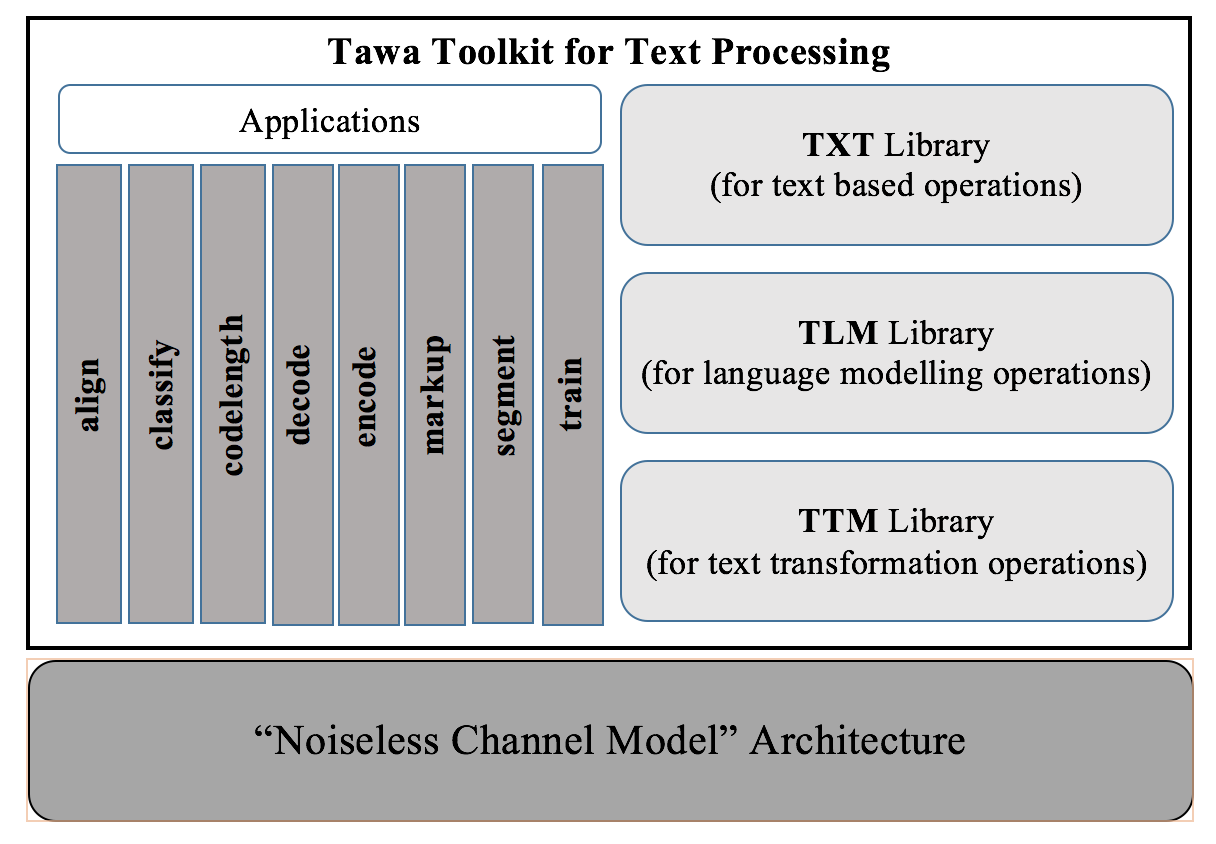
\includegraphics[height=4.5in,width=4.8in, keepaspectratio]{toolkit}
\caption{A diagrammatic overview of the Tawa Toolkit and its design.}
\label{figure:overall-design}
\end{figure}

The Noisy Channel Model is a common architecture for many NLP applications, such as OCR, spelling correction, POS tagging and machine translation~\cite{ker90}. In this architecture, applications are formulated as a communication process with the source text conceptualised as being sent down a communication channel by the sender, with the receiver trying to recover the original message in the presence of noise by correcting the observed text that is received. This process of text correction involves the search for the most probable corrected target text which is often referred to as decoding (see Figure~\ref{figure:architectures}a). Note that the correct source text is unknown---the search process for the target text makes a best guess as to what it might be.

\begin{figure}
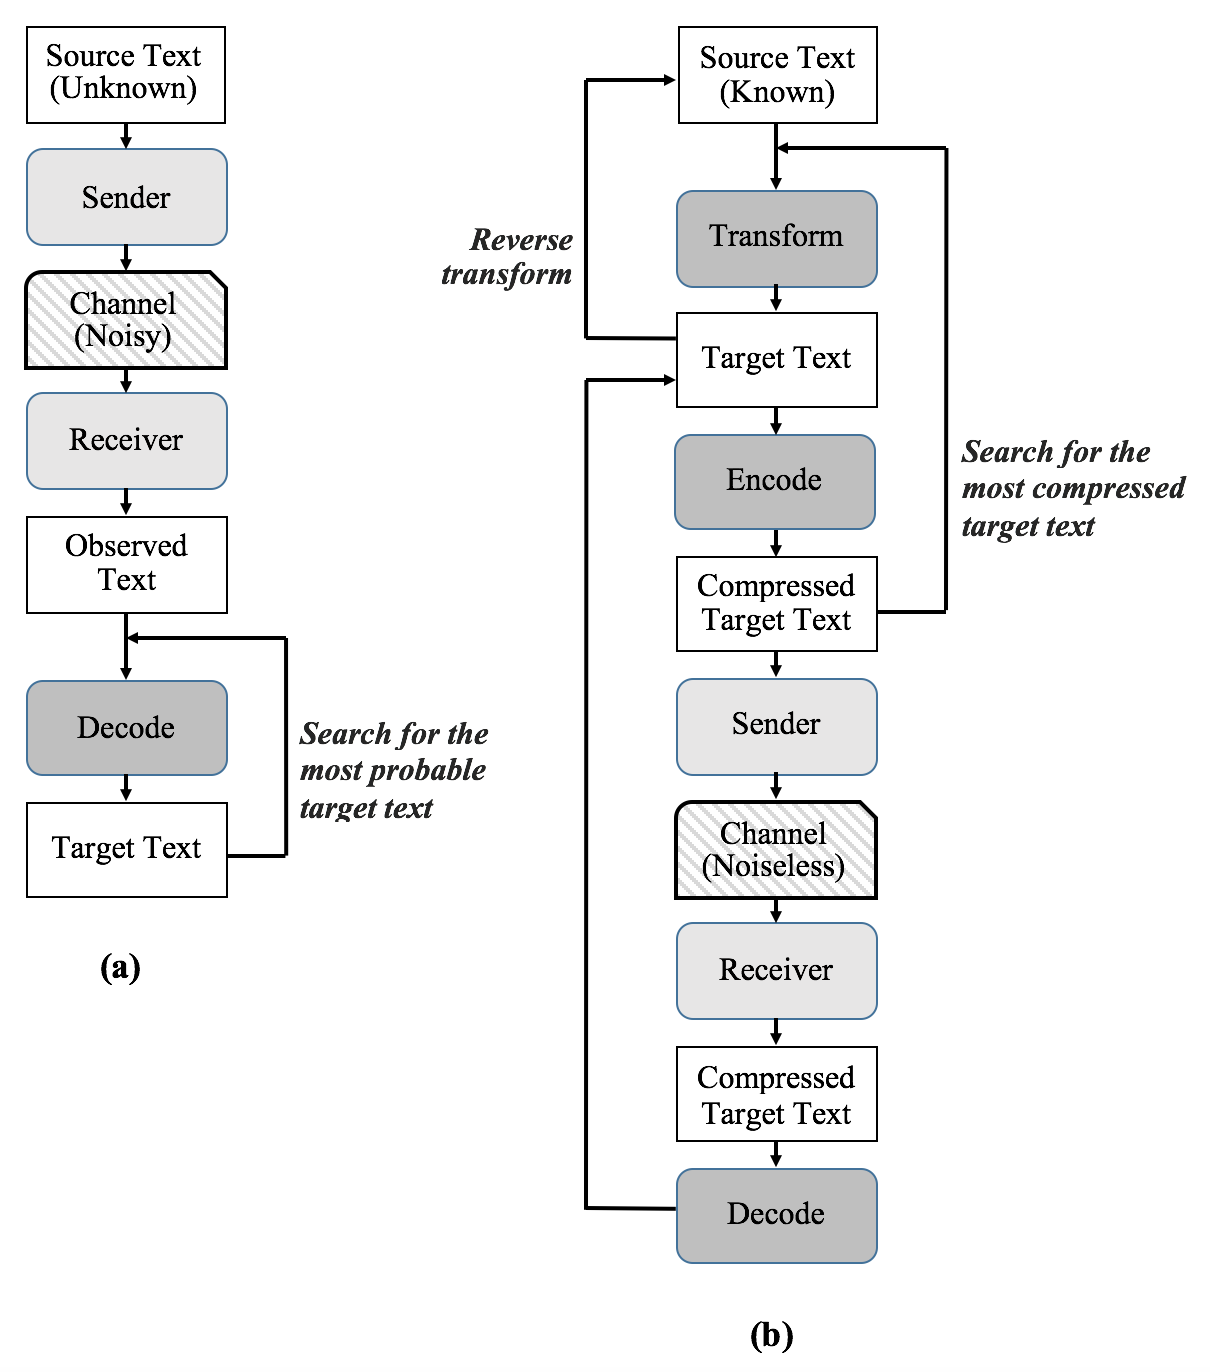
\includegraphics[height=5.5in,width=4.8in, keepaspectratio]{architectures}
\caption{Two architectures for NLP: (a) the standard decoding-based `Noisy Channel Model' versus (b) the encoding-based `Noiseless Channel Model' adopted by the Tawa Toolkit.}
\label{figure:architectures}
\end{figure}

The noisy channel model leads to robust and 
effective performance for many NLP tasks despite it being perhaps a rather arbitrary and abstract characterisation for NLP. As an alternative, we wish to adopt language models based on well performing text 
compression techniques such as PPM which have already been found to be highly effective in many NLP
applications~\cite{tea98,tea98a,tea00,tea00a,wit99a,wit99b,mah08}. Therefore, we have also
investigated in previous research~\cite{mah08} an alternative design perspective with an emphasis based on encoding rather than decoding. This has culminated in the architectural design shown in Figure~\ref{figure:architectures}b.
This design adheres to two main principles---the communication process must be both {\it lossless} and {\it reversible}. A lossless encoding by definition is reversible with no loss of information, with no noise being added to the message being transmitted. Note that any transformation that occurs prior to the encoding in our approach also needs to be reversible. This is so that there is
no loss in information during the communication in order to ensure the message is transmitted correctly and as efficiently as possible and this can be verified during decoding.

The Tawa toolkit based on this architecture has now gone through several design cycles culminating in the latest version of the toolkit described in this paper. In this updated toolkit, an NLP process is not thought of as being one of noisy communication, therefore requiring a  decoding process to recover the original message. Instead, the approach taken by the toolkit is to characterise an NLP process as a noiseless or noise-free communication. In this setting, the sender will search for the best encoding of the target message and this is then transmitted losslessly down the communication channel. In this case, the decoding process is of secondary importance, mainly  to verify the encoding process---the emphasis instead is placed on how efficiently the target message can be encoded. Also encoded is additional information on how to transform the source message into the target message. In this case, the search process---that of finding the best transformation, plus the information required to transform between them---occurs prior to the encoding phase rather than during the decoding phase. (See Figure~\ref{figure:architectures}b).

Following the workflow in the figure, the sender first starts from a known source text and transforms it in some way (as shown by the dark gray box labelled `Transform') into the target text. This is the text that is the desired output for some application (such as compression, text mining, spelling correction, machine translation and so on). In order to illustrate the variety of possible transformations which includes but goes beyond those traditionally covered by the noisy channel model, some example transformations are listed below\footnote{The first two examples above are transformations possible using a related tag insertion approach~\cite{yea01} that was similar to what was implemented in an earlier version of the toolkit. However, the subsequent examples above go beyond the tag insertion approach and are used to illustrate what is possible in the updated toolkit.}:

\begin{itemize}
\item inserting markup tags into the text (called tag insertion), such as to indicate where different languages are in the text for language segmentation~\cite{tea00a,alk17};
\item inserting extra characters, such as spaces for word segmentation~\cite{tea00};
\item changing the alphabet, such as replacing common character bigraphs or word bigrams with new symbols to aid
compression~\cite{tea98,alh14};
\item transforming the text into a grammar, such as for grammar-based compression~\cite{alj17};
\item encoding extra information such as parts-of-speech (POS) tags for POS tagging and tag-based compression~\cite{tea98,alk17a};
\item switching between models used to encode each symbol in the text~\cite{tea00a,tea01}.
\end{itemize}

The transformations are done in such a way that they are {\em reversible} (as shown by the line labelled `Reverse transform' in the figure). If tags or spaces are added, for example, then these can simply be removed to recover the original source text without any loss of information. If the alphabet is altered, then there is a one-to-one mapping between the old and new alphabets so that the original source text is easily recoverable. This property of reversibility ensures that information is communicated losslessly.

The target text is then encoded to produce the compressed target text (as depicted by the dark gray box labelled `Encode'). A search process shown in the figure by the rightmost arrow is used to find the most compressed text by repeatedly trying out different variations of the transformation (for example, by inserting or not inserting spaces after each character if performing word segmentation). This search
can be thought of as the transformation \& encoding phase whose purpose is to generate a suitable target text.

The remaining parts of the workflow shown in the figure is the verification \& decoding phase. This step is not necessarily needed depending on the application since just producing the target text will usually be sufficient in order to complete the task(s) required. However, as argued below, verification is of fundamental importance in ensuring the output is correct. This is done by sending the compressed target text down a noise-free communication channel, and then checking that the decoded target text matches the original target text.

Mahoui {\em et al}.~\shortcite{mah08} pointed out that the noiseless channel model could be viewed simply as ``the noisy channel model in another guise''. This is because the search processes (e.g. the Viterbi 
algorithm~\cite{vit67}) produce a similar result with the best target text being found in both cases. However, as Mahoui et al. have argued, there are important differences. Firstly, when designing text compression systems, it is well-known that the encoding and decoding processes are not  necessarily equivalent (for example, often either the encoding or decoding process can take noticeably longer as further effort is required to maintain probability tables in the form required for coding).

Secondly, the perspective has changed from correcting `noise' (which is just one approach to NLP) to one of efficiently encoding the source text plus further information to transform the message into the target text (which can be considered an equally plausible alternative approach to NLP).

Thirdly, as stated, the decoding process for the noiseless channel model provides a means for physically {\it verifying} the correctness of the communication. That is, we can directly apply standard techniques used for lossless text compression by checking that we can directly encode and decode the target message to and from a file on disk. (That is, there is a physical measurable object that exists in the real world). The noiseless channel model makes it clear that all information must be transmitted. Many current approaches using the noisy channel model base the decoding on implicit information and make the assumption that this information has little or no effect on the accuracy of the transformation. This may be correct, or erroneous, but this first needs to be verified, which is one of the main arguments for supporting the alternative approach in Figure~\ref{figure:architectures}b. All necessary information must be encoded explicitly otherwise it would not be possible to get the decoder to work.  As a consequence, the encoding codelengths (how much it takes in bits to physically encode the information) becomes a useful and verifiable means for measuring the effectiveness of the language  models being used.

And fourthly,  the changed perspective opens up further possibilities for improved language models based on models found effective for lossless text compression, such as: alternative encoding methods, not necessarily probabilistic, e.g. the Burrows Wheeler Transform~\cite{bw94} and Lempel-Ziv methods~\cite{zl77,zl78}; methods for preprocessing the text prior to encoding~\cite{at05,alh15}; and hybrid methods for combining or switching between models~\cite{vol98,tea01}.

It is also clear from  Figure~\ref{figure:architectures} that the source text for the noiseless channel model is known when it is encoded which contrasts with the noisy channel model where the original source text is unknown. This is a fundamental difference that must be considered when designing applications based on these two architectures. In the noisless case, the designer has access to all the information from the source text (since it is known) during the search which may be significantly more efficient as a result. For example, one method found effective at improving compression of natural language text is to replace common bigraphs with new single unique symbols prior to compression~\cite{alh15,alj17}. This is a very straightforward task for an encoder working from a known source to find the most common bigraphs. However, bigraph replacement at the decoding stage is not possible in the same way since the original source text is not known.

%\hl{Devise alternative diagrams, especially for preprocessing and postprocessing:}
%\begin{itemize}
%\item tokenisation
%\item preprocessing
%\item encoding
%\item decoding
%\item postprocessing
%\end{itemize}

\section{The toolkit's libraries}
\label{section.libraries}

In this section, the libraries provided with the toolkit are described.
As with the original Cleary and Teahan API~\shortcite{cle97} whose design the libraries are based upon,
the intention of the libraries is to shield the user from
details of the modelling and probability estimation process. A primary goal
is to allow the rapid prototyping of applications where the use of
textual models is needed, such as text compression, text classification, text mining, and text correction, with a minimal amount of code
needed for implementation.

\begin{table}
\centering
\begin{smaller}
\begin{tabular}{lp{10.2cm}} \hline
{\bf Object} & {\bf Description} \\ \hline 
{\it Symbol} &  A symbol is a number that is being modelled. It is represented in C as an unsigned int.
There is no notion of what a symbol means. However, it is restricted by the alphabet  size ($A$) when a model is created. e.g.
$A = 256$	is used for ASCII text;  $A = 0$ means an unbounded alphabet used for words.
The mapping between symbols and text characters is user-defined such as ASCII byte values or a different mapping (required for UTF-8 coded text). \\
{\it File} & A file is associated with a physical file on disk. It is used to open, read and load text files. \\
{\it Text} & A text is used for storing a sequence of symbols. They are essentially variable length arrays of symbols. \\ 
{\it Model} & A model provides predictions for sequences of symbols. It has an alphabet size ($A$) and order ($O$) associated with it. A model can also be static or dynamic. They are used for specifying the type of language model being used and the type of operations being performed (such as a PPM~\cite{cle84,mof90} language model).\\
{\it Coder} & A coder is used for encoding and decoding a sequence of symbols from compressed files on disk using an arithmetic coder, for example, or a range coder. \\
{\it Context} & A context is used for accessing and updating a model. The coding context is updated from the symbols that have just been encoded. (For a PPM model, the maximum length of the context is fixed as specified when the model is created).\\
{\it Transform} & A `transform' defines a possible transformation for altering or correcting the sequence. These are used for defining and performing transformations on the text such as used for correction-based or `tag insertion' style algorithms (i.e. insertion of markup tags). \\ \hline
\end{tabular}
\end{smaller}
\label{table.objects}
\caption{A summary of the objects used by the toolkit's libraries.}
\end{table}

Table~\ref{table.objects} lists the objects the libraries use and their description. When compared to standard text operations that
most programming languages provide, the $Symbol$ and $Text$ objects have a similar functionality to characters and strings, and the $File$ object is closely related to its programming language equivalent. However, the $Symbol$ object provides a much greater range of symbol numbers for the developer to use rather than just the 256 possibilities that 8-bit ASCII characters provide, for example, or even the range provided by Unicode characters. The maximum symbol number is defined by the \verb|TXT_max_symbol| method (for example, $2^{31}-3$ for PPM models in the current toolkit implementation). Although the
$Text$ object provides similar operations that strings do in standard programming languages, the length of the text is not restricted and
can be varied at run-time by some operations such as appending onto the end of the text.

The toolkit defines various further objects such as $Model$ and $Coder$ that facilitate the design of context-based modelling and compression-based applications and are used for specifying the `model' and `coder' that are at the heart of these types of compression applications. Rissanen and Langdon~\shortcite{rl81} have noted the important distinction between {\em modelling} and {\em coding}, and the toolkit uses this insight in its design. Uniquely, the toolkit also
explicitly incorporates a $Context$ object\footnote{This is similar to that used in pseudo-code for an adaptive statistic encoder and decoder proposed by Teahan~\shortcite{tea98}[page 112].}  as well in its design to aid in the traversal of the model and the probability estimation process as the text is processed sequentially.

The final $Transform$ is an object whose purpose is to ease the design of applications requiring some form of transformation on the text such as used for correction-based or `tag insertion' style algorithms (i.e. insertion of markup tags). The type of search algorithm, such as the Viterbi algorithm~\cite{vit67} or the stack decoding algorithm~\cite{jel69}, is specified when the $Transform$ object is created. Specific transformations of the form $source\ text  \rightarrow target\ text$ are then added to the object. These specify the source text sequence that must be matched before the target sequence is generated. Multiple transformations will generate multiple paths in the search tree. A similar convention used for regular expressions is used here  to represent (and match) the source and target text. For example: a wildcard form can be used to match any character; ranges denoted by [$\ldots$] denote character disjunction; and functions can also be used to match character sequences.
A method is used to start the transformation process using a specific $Model$ object to define what model to use for the encoding of the corrected target sequence and this can be called multiple times for different $Model$ objects. Another method is then called to perform the transformation process which returns a transformed $Text$ object upon completion which represents the most compressed transformed target sequence found by the search.

\subsection{A selection of methods provided by the toolkit's libraries}
\label{section.methods}

\begin{table}[h]
{\tabcolsep 0.70mm
\centering
\begin{smaller}
\begin{tabular}{llp{9.5cm}} \hline
{\bf Object} & {\bf Returns} & {\bf Method name and arguments} \\ \hline
{\it Symbol} & $Symbol$ & \verb|TLM_decode_symbol(|$Model$, $Context$, $Coder$\verb|)| \\
& $Void$ & \verb|TLM_encode_symbol(|$Model$, $Context$, $Symbol$, $Coder$\verb|)| \\
& $Void$ & \verb|TLM_find_symbol(|$Model$, $Context$, $Symbol$\verb|)|, \\
& $Symbol$ & \verb|TLM_max_symbol(|$Model$\verb|)|, \\ 
& $Boolean$ & \verb|TLM_next_symbol(|$Model$, $Context$, *$Symbol$\verb|)| \\ 
& $Boolean$ & \verb|TLM_reset_symbol(|$Model$, $Context$\verb|)| \\ 
& $Symbol$ & \verb|TXT_sentinel_symbol()| \\
{\it File} & $Void$ &\verb|TXT_close_file(|$File$\verb|)| \\
& $File$ & \verb|TXT_open_file(|$Filename$, $Mode$, ...\verb|)| \\
& $File$ & \verb|TXT_load_text(|$File$\verb|)| \\
& $Void$ &\verb|TXT_read_file(|$File$, $Text$, $Max$)\verb|| \\
& $Char$ &\verb|TXT_readline_file(|$File$, $Text$\verb|)| \\
& $Void$ & \verb|TXT_write_file(|$File$, $String$\verb|)| \\
{\it Text} & $Void$ & \verb|TXT_append_symbol(|$Text$, $Symbol$\verb|)| \\
& $Void$ &\verb|TXT_append_text(|$Text$, $Text1$\verb|)| \\
& $Text$ & \verb|TXT_create_text()| \\
& $Boolean$ & \verb|TXT_get_symbol(|$Text$, $Pos$, *$Symbol$\verb|)| \\
& $Boolean$ & \verb|TXT_is_alphanumeric(|$Symbol$\verb|)| \\
& $Boolean$ & \verb|TXT_is_ascii(|$Symbol$\verb|)| \\
& $Unsign.~Int.$ & \verb|TXT_length_text(|$Text$\verb|)| \\
& $Void$ &\verb|TXT_put_symbol(|$Text$, $Symbol$, $Pos$\verb|)| \\
& $Void$ &\verb|TXT_release_text(|$Text$\verb|)| \\
{\it Model} & $Model$ & \verb|TLM_create_model(|$ModelType$, $Title$, ...\verb|)| \\
& $Boolean$ &\verb|TLM_get_model(|$Model$, ...\verb|)| \\
& $Model$ &\verb|TLM_load_model(|$File$\verb|)| \\
& $Model$ &\verb|TLM_next_model()| \\
& $Unsign.~Int.$ &\verb|TLM_numberof_models()| \\
& $Void$ &\verb|TLM_release_model(|$Model$\verb|)| \\
& $Void$ &\verb|TLM_set_model(|$Model$, ...\verb|)| \\
& $Unsign.~Int.$ &\verb|TLM_sizeof_model(|$Model$\verb|)| \\
& $Void$ &\verb|TLM_reset_model()| \\
& $Void$ &\verb|TLM_write_model(|$File$, $Model$, $ModelForm$\verb|)| \\
{\it Coder} & $Coder$ &\verb|TLM_create_arithmetic_decoder(|$SourceFile$, $CompressedFile$\verb|) | \\
& $Coder$ &\verb|TLM_create_arithmetic_encoder(|$SourceFile$, $CompressedFile$\verb|) | \\
& $Void$ &\verb|TLM_release_coder(|$Coder$\verb|)| \\
{\it Context} & $Context$ &\verb|TLM_create_context(|$Model$\verb|)| \\
& $Void$ &\verb|TLM_release_context(|$Model$, $Context$\verb|)| \\
& $Void$ &\verb|TLM_update_context(|$Model$, $Context$, $Symbol$\verb|)| \\
{\it Transform} & $Void$ &\verb|TTM_add_transform(|$Transform$, $Codelength$, \\
& & ~~~$SourceFormatString$, $TransformFormatString$, ...\verb|)| \\
& $Transform$ &\verb|TTM_create_transform(|$TransformAlgorithm$, ...\verb|)| \\
& $Text$ &\verb|TTM_perform_search(|$Transform$, $SourceText$\verb|)| \\
& $Void$ &\verb|TTM_release_transform(|$Transform$\verb|)| \\
& $Void$ &\verb|TTM_start_search(|$Transform$, $Type$, $SourceText$, $Model$\verb|)| \\
\hline
\end{tabular}
\end{smaller}
\label{table.methods}
\caption{A selection of methods provided by the toolkit.}
}
\end{table}

Table~\ref{table.methods} provides a selection of the main methods provided by the libraries for each of the seven types of objects described in the previous section. Space precludes listing all the methods provided by the toolkit which can be found by downloading the software distribution.
The table lists methods for each object type in alphabetical order. The method name and its arguments are listed in column three of the table. Note that the prefixes \verb|TLM|, \verb|TXT| and \verb|TTM| used in the method names are used to signify the library being used for language modelling operations, text-based operations and transformation operations respectively. Column one lists the main type of object being operated upon, and column two lists the type of object returned by the method. (Here $Void$ indicates the method returns nothing, $Unsign.~Int.$ indicates the method returns an unsigned integer, $Transform$ a transform object, $Boolean$ a boolean and $Char$ a character with the other return types being one of the toolkit's object types). 

A brief description of these methods for each of the toolkit's object types now follows:

$\bullet$ Methods for $Symbol$ objects:
\verb|TLM_decode_symbol(|$Model$,$Context$,$Coder$\verb|)| returns the symbol decoded using the arithmetic $Coder$ and also updates the $Context$ for the $Model$ so that the last symbol in the context becomes the decoded symbol.
\verb|TLM_encode_symbol(|$Model$,$Context$,$Symbol$,$Coder$\verb|)| encodes the specified $Symbol$ using the arithmetic $Coder$ and also updates the $Context$ for the $Model$ so that the last symbol in the context becomes the encoded symbol.
\verb|TLM_find_symbol(|$Model$,$Context$,$Symbol$\verb|)| finds the predicted $Symbol$ in the $Context$ for the $Model$.
\verb|TLM_max_symbol(|$Model$\verb|)| returns the maximum symbol number allowed for the $Model$.
\verb|TLM_next_symbol(|$Model$,$Context$,*$Symbol$\verb|)| returns the next predicted $Symbol$ in the $Context$ for the $Model$ and the cost in bits of encoding it. The context is not updated. If a sequence of calls to \verb|TLM_next_symbol|
   are made, every symbol in the alphabet will be visited exactly once although the order in which
   they are visited is undefined being implementation and data dependent. The function   
   returns $False$ when there are no more symbols to process.                                                                               
   The codelength value that is returned is the same as that returned by \verb|TLM_update_context|     
   which may use a faster search method to find the symbol's codelength         
   more directly (rather than sequentially as \verb|TLM_next_symbol| does).
\verb|TLM_reset_symbol(|$Model$,$Context$\verb|)| resets the current position to point back at the first predicted symbol  
   in the $Context$ for the $Model$.
\verb|TXT_sentinel_symbol()| returns the ``sentinel symbol''. This is used where there is a break               
   required in the updating of the context, such as when the end of text has been reached or when more
   than one model is being used  to encode different parts of a text. The effect of encoding the  sentinel
   symbol is that the prior context is forced to the null string i.e. the subsequent context will contain just
   the sentinel symbol itself. This is useful during training if there are statistics that differ markedly at the
   start of some text than in the middle of it (for example, individual names, and titles within a long list).

$\bullet$ $File$ methods:
\verb|TXT_close_file(|$File$\verb|)|  closes the $File$ and releases memory used by the file object.
\verb|TXT_open_file(|$Filename$,$Mode$, ...\verb|)| opens the file named $Filename$ with the specified $Mode$ and creates and returns a file object for the file.
\verb|TXT_read_file(|$File$,$Text$,$Max$)\verb|| reads $Max$ symbols from the specified $File$ into the $Text$. If argument $Max$ is zero, then all symbols until $EOF$ are read.
\verb|TXT_readline_file(|$File$,$Text$\verb|)| loads the $Text$ using the next line of input from the $File$. Returns the       
   last character read or $EOF$.
\verb|TXT_write_file(|$File$,$String$\verb|)| writes out the $String$ to the $File$.

$\bullet$ $Text$ methods:
\verb|TXT_append_symbol(|$Text$,$Symbol$\verb|)| appends the $Symbol$ onto the end of $Text$.
\verb|TXT_append_text| appends $Text1$ onto the end of $Text$.
\verb|TXT_create_text()| creates and returns a text object for storing, accessing and updating a string of symbols.
\verb|TXT_get_symbol(|$Text$,$Pos$, *$Symbol$\verb|)| returns $True$ if there exists a symbol at position $Pos$ in the $Text$.  The argument $Symbol$ is set to the specified symbol if it exists.
\verb|TXT_is_alphanumeric(|$Symbol$\verb|)| returns $True$ if the $Symbol$ is an alphanumeric character.
\verb|TXT_is_ascii(|$Symbol$\verb|)| returns $True$ if the $Symbol$ is an ASCII character.
\verb|TXT_load_text(|$File$\verb|)| creates and returns a new text object, loading it using text from the $File$ (assuming standard ASCII text.
\verb|TXT_length_text(|$Text$\verb|)| returns the length of the $Text$.
\verb|TXT_put_symbol(|$Text$,$Symbol$,$Pos$\verb|)| inserts the $Symbol$ into the $Text$ at position $Pos$. Inserting a symbol beyond the current bounds of the text will cause a run-time error.
\verb|TXT_release_text(|$Text$\verb|)| frees the memory used by the $Text$.

$\bullet$ $Model$ methods:
\verb|TLM_create_model(|$ModelType$,$Title$, ...\verb|)| creates and returns a new empty dynamic model of the specified type $ModelType$,$Title$ (such as \verb|TLM_PPM_Model| for a PPM model) and other parameters depending on the $ModelType$.
\verb|TLM_get_model(|$Model$, ...\verb|)| returns information describing the $Model$ such as alphabet size and title.
\verb|TLM_load_model(|$File$\verb|)| loads a model which has been previously saved to the $File$ into memory and    
   allocates it a new model object which is returned.
\verb|TLM_next_model()| returns a model object for the next valid model in the list of models that have been loaded
into memory. Returns $Nil$ if there aren't any.
\verb|TLM_numberof_models()| returns the number of models currently loaded into memory.
\verb|TLM_release_model(|$Model$\verb|)| frees the memory used by the $Model$.
\verb|TLM_set_model(|$Model$, ...\verb|)| sets information that defines the $Model$ such as alphabet size and title.
\verb|TLM_sizeof_model(|$Model$\verb|)| returns the current number of bits needed to store the $Model$ in memory.
\verb|TLM_reset_model()| resets the current model so that the next call to \verb|TLM_next_model| will
return the first valid model in the list of models that have been loaded into memory (or $Nil$ if there are none).
\verb|TLM_write_model(|$File$,$Model$,$ModelForm$\verb|)| writes out the $Model$ to the $File$ (which can then be loaded by other applications later). The argument $ModelForm$ must have the value \verb|TLM_Static| or  \verb|TLM_Dynamic| and determines whether the model is static or dynamic when it is later reloaded using \verb|TLM_load_model|.

$\bullet$ $Coder$ methods:
\verb|TLM_create_arithmetic_decoder(|$SourceFile$, $CompressedFile$\verb|)| creates an arithmetic coder object used for decoding from the compressed file $CompressedFile$ back to the source file $SourceFile$.
\verb|TLM_create_arithmetic_encoder(|$SourceFile$,$CompressedFile$\verb|)| creates an arithmetic coder object used for encoding
from the source file $SourceFile$ to the compressed file $CompressedFile$.
\verb|TLM_release_coder(|$Coder$\verb|)| frees the memory used by the $Coder$.

$\bullet$ $Context$ methods:
\verb|TLM_create_context(|$Model$\verb|)| creates a context object for the $Model$ used during operations such as encoding, decoding and update on which predictions of the upcoming symbol are made.
\verb|TLM_update_context(|$Model$,$Context$,$Symbol$\verb|)| updates the $Context$ for the $Model$ using the current $Symbol$.
\verb|TLM_set_context_operation(|$Operation$\verb|)| sets the type of $Operation$ to be performed by the methods                   
   \verb|TLM_next_symbol|, \verb|TLM_find_symbol| and \verb|TLM_update_context| such as returning
   the codelength (in \verb|TLM_Codelength|) or a list of arithmetic coding ranges (in \verb|TLM_Coderanges|).               
\verb|TLM_release_context(|$Model$,$Context$\verb|)| frees the memory used by the $Context$ for $Model$.

$\bullet$ $Transform$ methods:
\verb|TTM_add_transform(|$Transform$,$Codelength$, $SourceFormatString$,$TransformFormatString$, ...\verb|)| adds the formatted correction to the $Transform$ object. The argument $SourceFormatString$
is the format of the original text begin corrected; $TransformFormatString$ is the format of the text it will be corrected to; and
$Codelength$ is the cost in bits of making that correction when the text is being corrected or marked up.
\verb|TTM_create_transform(|$TransformAlgorithm$, ...\verb|)| creates and returns a transform object which can be used to transform or ``mark up'' text.
The argument $TransformAlgorithm$ specifies the type of search algorithm to use such as \verb|TTM_Viterbi|.
\verb|TTM_perform_search(|$Transform$,$SourceText$\verb|)| creates and returns a text object that contains the result of the
search for the most compressible $SourceText$ when corrected according to the transform object and models associated with it.
\verb|TTM_release_transform(|$Transform$\verb|)| frees the memory used by the $Transform$.
\verb|TTM_start_search(|$Transform$,$Type$,$SourceText$,$Model$\verb|)| starts a new search process for correcting or marking up the $SourceText$ using the specified $Model$ by applying the transforms specified by the $Transform$. This routine must be called at least once before \verb|TTM_perform_search|. Multiple  calls to this procedure will cause separate transform paths to be initiated for each of the specified models.

\section{Sample applications provided by the toolkit}

\label{section.samples}

This section gives sample pseudo code for the following nine applications:

\begin{enumerate}
\item a method that encodes symbols using the PPM compression scheme (Algorithm~\ref{algo1});
\item a context based encoding method (Algorithm~\ref{algo2});
\item a context based decoding method (Algorithm~\ref{algo3});
\item a context based method for computing compression codelength without coding (Algorithm~\ref{algo4});
\item a context based method for building (``training'') models (Algorithm~\ref{algo5});
\item a compression-based method for text classification (Algorithm~\ref{algo6});
\item a compression-based method for verifying sentence alignment in a parallel corpus (Algorithm~\ref{algo7});
\item a compression-based method for performing word segmentation on a text file (Algorithm~\ref{algo8});
\item a compression-based method for performing language segmentation on a text file (Algorithm~\ref{algo9}).
\end{enumerate}

These examples are used to illustrate the use of common methods from the toolkit's libraries. Also, a further purpose of the examples is to illustrate the brevity of the solutions especially the algorithms for word segmentation and language segmentation considering the complexity of each of these applications which is hidden to the most extent from the developer.

\subsection{A PPM encoder}

The method \verb|PPMEncodeFile| as detailed in Algorithm~\ref{algo1} encodes symbols (such as bytes or characters) in an input file using the PPM compression scheme. The input file is passed to the method as the argument $SourceFile$ with the compressed output file specified by the argument $CompressedFile$. 

\begin{algorithm}[h!]
{\bf method} PPMEncodeFile ($SourceFile$, $CompressedFile$)\\

  $Model$ = TLM\_create\_model (TLM\_PPM\_Model,``Title'', 256, 5,``D'', $True$, $True$)\;
  $Coder$ = TLM\_create\_arithmetic\_encoder ($SourceFile$, $CompressedFile$)\;
  EncodeFile ($SourceFile$, $Model$, $Coder$)\;
  TLM\_release\_model($Model$)\;
  TLM\_release\_coder($Coder$)\;  
{\bf end}\\
\caption{A method for order 5 PPMD encoding.}
\label{algo1}
\end{algorithm}

The variable $Model$ specifies the model number of the PPM compression language model---this number is returned by the call to the routine \verb|TLM_create_model| for creating a new dynamic PPM model (line 2). The arguments to the call specify the model's title, that the alphabet size is 256, that the order of the model is 5, that escape method D is being used (that is, the model is PPMD), and that both full exclusions and update exclusions are being used. As an alternative, \verb|TLM_load_model| can be used to
load an existing static or dynamic model directly from disk rather than have it created as this method does.

The variable $Coder$ is set to the coder number of the arithmetic coder created for the method that is  returned
by the \verb|TLM_create_arithmetic_encoder| method (line 3). The coder is used to perform the arithmetic encoding and decoding used for encoding and decoding a stream of bits that represent the PPM model's predictions to a compressed file on disk.

Algorithm~\ref{algo1} calls the \verb|EncodeFile| method (line 4) which is defined in Algorithm~\ref{algo2} and described in the next subsection.
The method finishes by releasing the memory allocated to the $Model$ and $Coder$ that were created (lines 5 and 6). These release methods are necessary for implementations in programming languages that do not automatically free memory on exit of the method. Many of the objects used by the toolkit (such as the $Context$, $Model$, $Coder$ and $Transform$ objects) require complex multiple data structures for implementation and can take up considerable resources when many objects are created during Viterbi-style search operations, for example. Freeing up these resources is non trivial and dedicated methods for performing these operations are required and therefore explicitly defined by the toolkit.

\subsection{Context based encoding and decoding}

Algorithms~\ref{algo2} and~\ref{algo3} provides pseudo-code for context-based encoding and decoding of a file respectively. They assume that a $Model$ has already been created or loaded and a $Coder$ has been created prior to these methods being called with these being passed as arguments. The encoder requires the input file ($SourceFile$) as an argument, and the decoder requires the compressed file ($CompressedFile$) as an argument.

\begin{algorithm}[h!]
{\bf method} EncodeFile ($SourceFile$, $Model$, $Coder$)\\
  $Context$ $\gets$ TLM\_create\_context ($Model$)\;
  \For {each $Symbol$ in $SourceFile$}{
    TLM\_encode\_symbol ($Model$, $Context$, $Symbol$, $Coder$)
  }
  TLM\_encode\_symbol ($Model$, $Context$, $Coder$, TXT\_sentinel\_symbol())\;
  TLM\_release\_context ($Context$)\;
  {\bf end}\\
\caption{A context based method for encoding.}
\label{algo2}
\end{algorithm}

\begin{algorithm}[h!]
{\bf method} DecodeFile ($CompressedFile$, $Model$, $Coder$)\\
  $Context$ $\gets$ TLM\_create\_context ($Model$)\;
  \While {$Symbol \gets$ TLM\_decode\_symbol ($Model$, $Context$, $Coder$) != TXT\_sentinel\_symbol()}{
    Output $Symbol$
  }
  TLM\_release\_context ($Context$)\;
{\bf end}\\
\caption{A context based method for decoding.}
\label{algo3}
\end{algorithm}

Both methods require that a $Context$ variable be created first using the \verb|TLM_create_context| method (lines 2). Then each symbol is processed sequentially, either encoded using the \verb|TLM_encode_symbol| method (line 4, Algorithm~\ref{algo2}) or decoded using the \verb|TLM_decode_symbol| method (line 3, Algorithm~\ref{algo3}). (These methods also update the $Context$ at the same time for the current symbol. The $Context$ is released just before the end of both methods).

Both methods process symbols sequentially which is specified using the variable $Symbol$.
The way a file is preprocessed (during encoding) and postprocessed (during decoding) is user-defined. Symbols for English text are usually mapped directly to the ASCII byte values of the characters in the file. For Unicode (e.g. UTF-8) encoded files, on the other hand, a different mapping is required. Further preprocessing / postprocessing of the symbol stream may also be performed such as replacement of common bigraphs~\cite{tea98,alh14,alj17} (also see Section~\ref{section.results} below) as this can often lead to improved compression. However, these steps are not detailed in Algorithms~\ref{algo2} and~\ref{algo3}.

The special sentinel symbol (returned by \verb|TXT_sentinel_symbol|) has been used to signify the end of the encoding stream and is encoded once all the other symbols in the file have been encoded (line 6, Algorithm~\ref{algo2}). It is a unique character which effectively expands a model's alphabet by one that is encoded at the end of an encoding stream and forces the model to back off to the default oder -1 context. The decoder simply decodes symbols until the sentinel symbol is decoded (line 3, Algorithm~\ref{algo3}). An alternative way of encoding the end of the stream which the toolkit implements is to encode the length of the stream at the beginning using (for example) a start-stop-step encoder~\cite{bcw90}. However, this requires a first pass through the stream being encoded to find its length, and using a unique extra symbol such as \verb|TXT_sentinel_symbol| does not incur much overhead except for the cost of the escapes down to the order -1 context and the cost of encoding this symbol in the lowest order context which is ameliorated by PPM's full exclusions mechanism.

\subsection{Calculating compression codelengths without coding}

The method \verb|CodelengthText| in Algorithm~\ref{algo4} calculates the compression codelength for a text object without performing any coding operation. It is similar to the
encoding and decoding methods above, except that it uses the routine
\verb|TLM_update_context| to update the model (line 5) instead of either \verb|TLM_encode_symbol| or
\verb|TLM_decode_symbol| as above. 
The argument $Model$ specifies the language model
being used. The text $SourceText$ passed as an argument would usually have the sentinel symbol marking the end of the text so therefore this does not need to be explicitly processed at the end of the stream (as was the case with Algorithm~\ref{algo2}).
The variable $Codelength$ (line 2) is used to accumulate the totals of the compression codelengths as each symbol in the text is processed. It is returned by the method at the end (line 9). The codelength values that are the cost of encoding each symbol are obtained by accessing the variable \verb|TLM_codelength| (see line 6) and reflect the theoretically optimum encoding of each symbol for which the actual (physical) encoding to disk using an arithmetic coder is a very close approximation~\cite{rl79,wit87}. This method can be used to speed up processing as it does not perform any physical coding and has wide applications. A variant of the algorithm has been used to perform the automatic cryptanalysis of transposition ciphers, for example~\cite{alk16}.


\begin{algorithm}[h!]
{\bf method} CodelengthText ($SourceText$, $Model$)\\
  $Codelength \gets$ 0.0\;
  $Context \gets$ TLM\_create\_context ($Model$)\;
  \For {each $Symbol$ in $SourceText$}{
    TLM\_update\_context ($Model$, $Context$, $Symbol$)\;
    $Codelength$ += TLM\_Codelength\;
  }
  TLM\_release\_context ($Context$)\;

  \Return {$Codelength$}\;
{\bf end}\\
\caption{A context based method for computing compression codelength without coding.}
\label{algo4}
\end{algorithm}

\subsection{Building models}

The method \verb|TrainFile| in Algorithm~\ref{algo5} builds (or `trains') a model from the text in the file $SourceFile$ passed as an argument.
The way the algorithm works is similar to Algorithm~\ref{algo5} above as it uses \verb|TLM_update_context| (line 4) to process each
symbol sequentially (line 3) without performing any coding. However, no codelength calculations need to be performed in this case since all we are doing is building a model.

\begin{algorithm}[h!]
{\bf method} TrainFile ($SourceFile$, $Model$, $ModelType$, $ModelFilename$)\\
  $Context$ $\gets$ TLM\_create\_context ($Model$)\;
  \For {each $Symbol$ in $SourceFile$}{
    TLM\_update\_context ($Model$, $Context$, $Symbol$)
  }
  TLM\_update\_context ($Model$, $Context$, TXT\_sentinel\_symbol())\;
  TLM\_release\_context ($Context$)\;

  TLM\_write\_model ($ModelFilename$, $Model$,  $ModelType$)\;
{\bf end}\\
\caption{A context based method for building models.}
\label{algo5}
\end{algorithm}

The method can be used to build a dynamic model (which keeps on being updated when further files are processed at a latter time) or a
static model (which does not subsequently change and therefore will always give the same probability estimates). This explains the
need for the argument $Model$ to specify an already existing model which may be dynamic. (It will have been initially created using a call to \verb|TLM_create_model| similar to that on line 2 in Algorithm~\ref{algo1}). The argument $ModelType$ specifies whether the model
is dynamic or static. The model is written out to the file named $ModelFilename$ (using the call to \verb|TLM_write_model| on line 8) and can be latter loaded directly using a call to \verb|TLM_load_model| without the need for symbol processing. (Note that the size of a model, such as a PPM model, will usually be significantly smaller than the size of the text used to train it, even for higher order models).

Once a dynamic model is written out as a static model, it can not be subsequently updated. The use of static models can lead to better performance in some tasks (such as text classification) and optimisation of model memory allocation and data structures can be performed once it is known that the model will not be updated in the future.

Usually the symbols in the text will be processed directly from the source training file (from $SourceFile$) rather than from an intermediate
text ($SourceText$). For example, in the following text classification application, compression codelength calculations for multiple
models need to be performed on the same source file, and therefore it is more efficient to load the source file once into a text object
and have it available for subsequent processing without the need for further I/O operations being performed on the same file.

\subsection{Text classification}

The method \verb|ClassifyFile| in Algorithm~\ref{algo6} performs text classification on a text file. It classifies the file $SourceFile$ by finding which model compresses the text in the file best. This symbol-based method of text classification has been found to be competitive in many classification tasks compared to standard feature-based (word) classification schemes often with state-of-the-art results~\cite{tea03}. It has been used to accurately identify the natural language in which the source text is written~\cite{kt03}, and to identify the
most likely author of the text~\cite{tea01}, for example. Recent results have shown that it can classify gender~\cite{alt17}, recognise emotions~\cite{alm17} and even identify whether the text has been written by a person who is dyslexic or not~\cite{ala17}.

\begin{algorithm}[h!]
{\bf method} ClassifyFile ($SourceFile$)\\
  $BestCodelength \gets$ 0.0\;
  $BestModelTitle \gets$ NULL\; 
  $SourceText \gets$ TXT\_load\_text ($SourceFile$)\;
  TLM\_reset\_model ()\;
  \While {$Model \gets$ TLM\_next\_model $()$}{
      $Codelength \gets$ CodelengthText ($SourceText$,$Model$)\;
      \uIf {$(BestCodelength$ = $0.0)$ {\bf or} $(Codelength$ $<$ $BestCodelength)$}
         { $BestCodelength \gets Codelength$\;
           $BestModelTitle \gets$ TLM\_get\_title ($Model$);}
   }
  TXT\_release\_text ($SourceText$)\;

  \Return{$BestModelTitle$}\;
{\bf end}\\
\caption{A compression-based based method for text classification.}
\label{algo6}
\end{algorithm}

The method calls \verb|TLM_reset_model| and \verb|TLM_next_model| to cycle through all the models that have previously been loaded into memory (lines 5 and 6). The compression codelength is calculated on line 7 by calling the \verb|CodelengthText| method that was defined in Algorithm~\ref{algo4}. \verb|TXT_load_text| is used to load the source file once into the text object $SourceText$ (line 4). Note that \verb|TXT_load_text| appends the sentinel symbol onto the end of the text.

The method works by cycling through all the models to compute their compression codelengths on the source text, and returns the
title (obtained using the call to \verb|TLM_get_title| on line 10) of the best performing model.

\subsection{Verifying sentence alignment of a parallel corpus}

The method \verb|VerifyParallelFiles| in Algorithm~\ref{algo7} checks the quality of sentence alignment between two files ($File${\it 1} and $File${\it 2}) in a parallel corpus. It assumes that the corpus has already been aligned and the purpose of this method is to verify its quality prior to being used to build language models for statistical machine translation. The method also assumes that the sentences in the two different languages are on corresponding separate lines in the two files. Therefore, the \verb|TXT_readline_file| (line 5) is being used to read each line of the two files simultaneously into two text objects $Text{\it 1}$ and $Text{\it 2}$.

\begin{algorithm}[h!]
{\bf method} VerifyParallelFiles ($File${\it 1},$File${\it 2}, $Model${\it 1}, $Model${\it 2}, $CRThreshold$)\\

  $Text{\it 1} \gets$ TXT\_create\_text ()\;
  $Text{\it 2} \gets$ TXT\_create\_text ()\;
  
  $LineNo \gets 0$\;
  \While {TXT\_readline\_file ($File${\it 1}, $Text{\it 1}$) {\bf and} TXT\_readline\_text ($File${\it 2}, $Text{\it 2}$)} {
    $LineNo \gets LineNo + 1$\;
    $Codelength{\it 1} \gets$ CodelengthText ($Text{\it 1}$,$Model${\it 1})\;
    $Codelength{\it 2} \gets$ CodelengthText ($Text{\it 2}$,$Model${\it 2})\;
    \uIf {$Codelength{\it 1} > Codelength{\it 1}$}
      { $CR \gets Codelength{\it 1} / Codelength{\it 2}$ }
    \uElse
      { $CR \gets Codelength{\it 2} / Codelength{\it 1}$ }
    \uIf {$CR > CRThreshold$}
      { Output ``Check alignment for Line '' $LineNo$ }
  }

  TXT\_release\_text ($Text{\it 1}$)\;
  TXT\_release\_text ($Text{\it 2}$)\;
{\bf end}\\
\caption{A compression-based method for verifying parallel sentence alignment.}
\label{algo7}
\end{algorithm}

The method \verb|CodelengthText| from Algorithm~\ref{algo4} is used to calculate the compression codelengths of the two sentences
in $Text{\it 1}$ and $Text{\it 2}$ according to the models $Model{\it 1}$ and $Model{\it 2}$ respectively. In order for this method to be effective, it requires the two models to be separately trained on a large amount of text that is representative of the respective languages.
Recent research~\cite{liu14,slt15} has shown that comparing compression codelength in this manner is an effective way for verifying that corresponding sentences are aligned, as well as measuring the quality of translation.

The method specifically computes the codelength ratio ($CR$) measure on lines 9 to 12 which is the maximum of the two ratios
$Codelength{\it 1} / Codelength{\it 2}$ and $Codelength{\it 2} / Codelength{\it 1}$. This ensures that $CR$ is always greater than
or equal to 1.0. A value of 1.0 indicates that the two codelengths are the same value and values close to or equal to 1.0 provide strong evidence that the sentences are probably aligned. This is based on the assumption that the information (from an information theoretical sense) between corresponding sentences that are co-translations should be the same or similar, and compression codelength provides an excellent means for measuring the information~\cite{liu14}.

The method on line 13 compares $CR$ to a threshold $CRThreshold$ which is passed as an argument. If $CR$ exceeds this threshold, then a message is output with the line number of the suspicious sentence (line 14). Values of 1.8 and above for $CRThreshold$ have been found effective at locating unsatisfactory translations in experiments with Chinese/English~\cite{liu14} and Arabic/English~\cite{slt15} parallel corpora. These experiments also show that codelength based measurements are more effective than sentence length based measurements for verifying sentence alignment.


\subsection{Word segmentation}

The method \verb|WordSegmentlFile| in Algorithm~\ref{algo8} performs word segmentation on the file $SourceFile$. Specifically,
it will insert spaces into the file which usually contains no spaces to indicate where the words are. Word segmentation is an important NLP application for languages that are not naturally word segmented such as Chinese. The method shown
in Algorithm~\ref{algo8} is based on the PPM-based word segmentation method~\cite{tea00} that has been used as a baseline model for an international evaluation on Chinese word segmentation~\cite{spr03}.

\begin{algorithm}[h!]
{\bf method} WordSegmentFile ($SourceFile$, $Model$, $Alphanumeric?$)\\

  $SourceText \gets$ TXT\_load\_text ($SourceFile$)\;

  $Transform \gets$ TTM\_create\_transform (TTM\_Viterbi)\;
  TTM\_add\_transform ($Transform$, 0.0, ``\%w'', ``\%w'')\;
  \uIf {{\bf not} $Alphanumeric?$}
    { TTM\_add\_transform ($Transform$, 0.0, ``\%w'', ``\%w~~'')\;}
  \uElse
    { TTM\_add\_transform ($Transform$, 0.0, ``\%f'', ``\%f~~'', TXT\_is\_aplhanumeric)\;}


  TTM\_start\_transform ($Transform$, $TransformType$, $SourceText$, $Model$)\;
  $TransformText \gets$
      TTM\_perform\_transform ($Transform$, $SourceText$)\;

  TTM\_release\_text ($SourceText$)\;
  TTM\_release\_transform ($Transform$);

  \Return{$TransformText$}\;
{\bf end}\\
\caption{A compression-based method for word segmentation.}
\label{algo8}
\end{algorithm}

The method uses a transform object $Transform$ to perform the segmentation. It is created on line 3 using \verb|TTM_create_transform| which specifies that the Viterbi search algorithm be used to find the best segmentation (as measured by the sequence of text with spaces inserted which has the lowest compression codelength). The method then specifies using \verb|TTM_add_transform| that two transformations be used for the search (lines 4 to 8). This defines the cost of the transformation in codelength (second argument to \verb|TTM_add_transform|), the symbol sequence that needs to be matched (third argument) specified using a \verb|printf|-like string syntax borrowed from the C programming language, and the transformed sequence (fourth argument) also specified using \verb|printf|-like string syntax. The first transformation added to the transform model in the method on line 4 specifies that whatever the current symbol is (using the wildcard ``\%w'' for the third argument to indicate that any symbol should be matched), it should always be included unchanged as one pathway in the search tree. This is because the wildcard ``\%w'' is also being used for the fourth argument meaning that whatever symbol matches it should be transformed unchanged. Line 4 is typically found in
most transform-based applications since usually the original text symbols need to form one search pathway rather than be totally discarded and/or transformed into something else.

The method uses the argument $Alphanumeric?$ to indicate which of the second transformations (line 6 or line 8) should be applied to the search. If this argument is not true, then a space symbol is inserted prior to each symbol (there is a space included at the beginning of the transformed sequence ``~~\%w'' for the fourth argument on line 6). This transformation would typically be used for word segmentation of Chinese text, for example, since in this case, we would wish to search through all the possible insertions of spaces after each of the symbols in the text. If the argument $Alphanumeric?$ is true, on the other hand, the transformation on line 8 specifies that spaces only be inserted after alphanumeric characters as a possible search pathway (using the ``~~\%f'' option for the matching and transformed sequences to specify that the function \verb|TXT_is_alphanumeric| be used to match the symbol). This transformation is a useful optimisation if English text without spaces is being segmented (by finding where to put the spaces back) since it will substantially reduce the search as non-alphanumeric characters will remain unchanged and not cause an extra pathway to be added to the search tree.

The effect of having two transformations used in this method is that two search pathways will be generated for every symbol being transformed. Hence, the maximum size of the search tree is essentially $2^n$ where $n$ is the number of symbols being transformed. The search is started using \verb|TTM_start_search| on line 9 which initialises the search for the best transformation of the $SourceText$ using the $Model$.  The Viterbi algorithm that is executed by the \verb|TTM_perform_search| operation (line 10) substantially reduces this search using trellis-based techniques and other optimisations so that for Markov-based models (such as PPM models) the search is completed essentially in linear time. The method returns the transformed text $TransformText$ which has the best compression codelength compared to alternatives once the search performed by \verb|TTM_perform_search| has been completed.

\subsection{Language segmentation}

The method \verb|LanguageSegmentlFile| in Algorithm~\ref{algo8} performs language segmentation. That is, it marks the boundaries between different languages in the same file. This is an important NLP application for texts that contain multiple languages which aren't explicitly marked up, and also for languages where code-switching is common, for example Arabic and Welsh, as an important early
step that should be performed on the NLP pipeline.

\begin{algorithm}[h!]
{\bf method} LanguageSegmentFile ($SourceFile$)\\

  $SourceText \gets$ TXT\_load\_text ($SourceFile$)\;

  $Transform \gets$ TTM\_create\_transform (TTM\_Viterbi)\;
  TTM\_add\_transform ($Transform$, 0.0, ``\%w'', ``\%w'')\;
  TLM\_reset\_model ()\;
   \While {($Model \gets$ TLM\_next\_model ())}
      { TTM\_add\_transform ($Transform$, 0.0, ``\%w'', ``\%m\%w'', $Model$)\; }

   TLM\_reset\_model ()\;
   \While {($Model \gets$ TLM\_next\_model ())}
       { TTM\_start\_transform ($Transform$, $TransformType$, $SourceText$, $Model$)\; }

  $TransformText \gets$
      TTM\_perform\_transform ($Transform$, $SourceText$)\;

  TTM\_release\_text ($SourceText$)\;
  TTM\_release\_transform ($Transform$);

  \Return{$TransformText$}\;
{\bf end}\\
\caption{A compression-based method for language segmentation.}
\label{algo9}
\end{algorithm}

The method creates a transform object $Transform$ on line 3 and specifies that the Viterbi algorithm be used to perform the search
for the best transformation. The method then adds a transformation using \verb|TTM_add_transform| on line 4 that uses the wildcard ``\%w'' form to ensure that the current symbol unchanged is included as one of the search pathways. Then the ``\%m'' form is inserted as
an alternative pathway for each model that has been loaded into memory (lines 5 to 8). This form states that for the transformed text, the model which is passed as the argument to \verb|TTM_add_transform| on line 7 will be used to predict subsequent symbols in the transformed text.

As with the previous word segmentation in Algorithm~\ref{algo8}, the effect of having the transformations used in this method is that multiple search pathways will be generated for every symbol being processed. In this case, all possible segmentations of the text using the models that have been loaded will be searched. Hence, the maximum size of the search tree in this case is $m^n$ where $m$ is the number of models used and $n$ is the length of the text. The search for the best transformation of the $SourceText$ is started using \verb|TTM_start_search| for each model on line 11.  Again, the Viterbi algorithm which is executed by \verb|TTM_perform_search| (line 13) substantially reduces the search using trellis-based techniques and other optimisations and the method returns the transformed text $TransformText$ which has the best compression codelength once the search has been completed.

\subsection{Applications implemented by the toolkit}
\label{section.applications}

The algorithms detailed above have all been implemented using the Tawa toolkit's libraries in the C programming language.
Table~\ref{table.apps} summarises these applications that come bundled with the toolkit. The table lists for each application its name (in 
bold font), a short description (in bold and italic fonts), the algorithms detailed above they are based on and selected arguments. The {\bf encode}, {\bf decode} and {\bf train} applications for PPM compression, decompression and model building, for example, use similar arguments which specify amongst other things the argument size, order of the model, and whether the model performs full exclusions and update exclusions. The  {\bf train} application has additional arguments for specifying the title of the model, and whether the model should be written out as a static model. The {\bf markup} and {\bf segment} applications use arguments for specifying whether Viterbi search should be adopted, and the stack depth if the stack algorithm should be used instead.

These application arguments provide a wide range of possible settings that have proven to be very effective in many NLP experiments as summarised in Section~\ref{section.results}. Many further possible uses still exist for these applications which have the advantage that they can be used ``off-the-shelf'' without the need to perform any further development using the toolkit's libraries.

\begin{table}
\small
\centering
\begin{tabular}{lp{12.0cm}} \hline
\multicolumn{2}{l}{{\bf align --} \textbf {\textit {tool for verifying sentence alignment}} (based on Algorithm 7)} \\
~ & \verb|-1 fn| ({\it fn = parallel text filename for language 1})
\verb|-2 fn| ({\it fn = parallel text filename for language 2})
\verb|-3 fn| ({\it fn = model filename for language 1})
\verb|-4 fn| ({\it fn = model filename for language 2}) \\
\hline
\multicolumn{2}{l}{{\bf classify --}  \textbf {\textit {tool to classify text files}}  (uses Algorithm 4 and 6)} \\
~ & \verb|-m fn| ({\it fn = filename for list of models})
\verb|-t fn| ({\it fn = filename for list of test files}) \\
\hline
\multicolumn{2}{l}{{\bf codelength --}  \textbf {\textit {writes out compression codelengths}} (uses Algorithm 4 and 6)}  \\
~ & \verb|-c| ({\it print outs codelengths for each character})
\verb|-e| ({\it calculates cross-entropy and not codelength})
\verb|-m fn| ({\it fn = filename for list of models}) \\
\hline
\multicolumn{2}{l}{{\bf decode --}  \textbf {\textit {PPM decoder (decompression tool)}} {\bf ~\&} (uses Algorithm 3)} \\
\multicolumn{2}{l}{{\bf encode --}  \textbf {\textit {PPM encoder (compression tool)}} (uses Algorithms 1 and 2)} \\
~ & \verb|-a n|	({\it n = size of alphabet})
\verb|-e c|	({\it c = escape method for the model})
\verb|-F| ({\it does not perform full exclusions})
\verb|-m fn| ({\it fn = model filename})
\verb|-N| ({\it input is unsigned integers})
\verb|-O n| ({\it n = max order of model})
\verb|-p n| ({\it report progress every n symbols})
\verb|-U| ({\it does not perform update exclusions}) \\
\hline
\multicolumn{2}{l}{{\bf markup --}  \textbf {\textit {segments a file by languages}} (uses Algorithm 9)} \\
~ & \verb|-D n| ({\it n = stack depth}) 
\verb|-m fn| ({\it fn = model filename})
\verb|-V| ({\it Use Viterbi algorithm}) \\
\hline
\multicolumn{2}{l}{{\bf segment --}  \textbf {\textit {segments a file by words}} (uses Algorithm 8)} \\
~ & \verb|-A| ({\it Alphanumeric characters only})
\verb|-D n| ({\it n = stack depth}) 
\verb|-m fn| ({\it fn = model filename})
\verb|-N| ({\it input is unsigned integers})
\verb|-V| ({\it Use Viterbi algorithm}) \\
\hline
\multicolumn{2}{l}{{\bf train --}  \textbf {\textit {builds PPM models}} (uses Algorithm 5)} \\
~ & {\it same arguments as for} {\bf encode} and {\bf decode} {\it plus:} \\
~ & \verb|-S| ({\it writes out the model as a static model})
\verb|-T str| ({\it title of the model}) \\
\hline
\end{tabular}
\caption{Applications implemented by the Tawa toolkit with selected arguments.}
\label{table.apps}
\end{table}

\begin{table}
\small
\begin{tabular}{lp{12.0cm}} \hline
1 & \verb|encode -a 256 -O 5 <Brown.txt >Brown.encoded| \\
   & \verb|bytes input 5998525 bytes output 1613517 2.152 bpc| \\
2 & \verb|decode -a 256 -O 5 <Brown.encoded >Brown.decoded| \\
3 & \verb|diff Brown.decoded Brown.txt| \\
4 & \verb|train -S -a 256 -O 5 -e D -T "Brown model" <Brown.txt >Brown.model| \\
   & \verb|Trained on 5998525 symbols| \\
5 & \verb|encode -m Brown.model <LOB.txt >LOB.encoded| \\
   & \verb|bytes input 5877271 bytes output 1609902 2.191 bpc| \\
6 & \verb|encode -a 256 -O 5 <LOB.txt >/dev/null| \\
   & \verb|bytes input 5877271 bytes output 1565250 2.131 bpc| \\
7 & \verb|codelength -e -m models.txt <Brown.txt| \\
   & \verb|English                      3.514| \\
   & \verb|French                       5.421| \\
   & \verb|German                       5.618| \\
   & \verb|Italian                      5.664| \\
   & \verb|Latin                        5.400| \\
   & \verb|Maori                        5.820| \\
   & \verb|Spanish                      5.602| \\
   & \verb|Minimum cross-entropy for English =     3.514| \\
8 & \verb|segment -m Brown.model -V -i woods_unsegm.txt -o woods_segm.txt| \\
9 & \verb|diff woods_segm.txt woods_correct.txt| \\
   & \verb|< Of easy wind and down yflake| \\
   & \verb|> Of easy wind and downy flake| \\
10& \verb|markup -m models.txt <e_and_m.txt -V -F| \\
   & \verb|<Maori>TE MANUHIRI TUARANGI <\Maori><English>AND MAORI INTELLIGENCER| \\
   & \verb|LET THE PAKEHA AND THE MAORI BE UNITED.| \\
   & \verb|Salutations to you friends the Maori people of New Zealand!  Chiefs and| \\
   & \verb|commoners, great and small, old and young salutations to you all !| \\
   & \verb|It is customary among the Maories to welcome the advent of a stranger With| \\
   & \verb|cries of <\English><Maori>Haere mai! Haere mai! <\Maori><English>| \\
   & \verb|The welcome is commenced with the approach| \\
   & \verb|of the visitor, and is prolonged until he has fairly entered the Kainga,| \\
   & \verb|Now therefore, the <\English><Maori>Manuhiri Tuarangi <\Maori><English>| \\
   & \verb|awaits the welcome of the Maori people.| \\
\hline
\end{tabular}
\caption{Sample commands and output using applications implemented by the toolkit.}
\label{table.commands}
\end{table}

Some examples of shell commands and output using these applications are shown in Table~\ref{table.commands}. The purpose of including these here is to demonstrate typical use and also some of the possibilities offered by the commands. Line 1 provides an
example of typical use for the {\bf encode} application. In this case the raw text from the million word Brown corpus of American English~\cite{fra79} in the file \verb|Brown.txt| is being encoded (compressed) to the file \verb|Brown.encoded| using the order 5 PPMD algorithm (which is the default) with an alphabet of 256. Some summary data is output when the program completes such as the number of input bytes, the number of output bytes and the compression ratio of 2.152 bpc (bits per character). Line 2 provides the command that can be used to decode (decompress) the encoded file, and the \verb|diff| command on Line 3 confirms that the decoded file is the same as the original file since no differences are produced as output.

Line 4 provides an example of how the {\bf train} command can be used to build a model. In this case, the Brown corpus is being used to train a static order 5 PPMD model which is written out to the file \verb|Brown.model| when the command completes. Line 5 loads the model direct into memory (without the need for processing the original training text which is much slower), and then uses it to encode another text, the raw text from the million word LOB corpus of British English~\cite{joh86} in the file \verb|LOB.txt| with a compression ratio of 2.191 bpc for the encoded output file \verb|LOB.encoded|. Line 6
encodes the LOB corpus directly without loading a model, therefore will use a dynamic model that adapts to the text being encoded
(i.e. at the beginning, the model is empty but is updated as the text is processed sequentially).  The compression ratio of 2.131 for this
adaptive approach is slightly better than the static approach used in Line 5 despite the dynamic model being empty at the start. This is a typical result for PPM models and reflects the effectiveness of these models at adapting quickly to the specific nature of the text. Also, the earlier language in the source document (British English in this case from the LOB corpus) is often a better predictor of subsequent text in the same document rather than using some other source to prime the encoding model in advance (American English from the Brown corpus).

Line 7 provides an example of the use of the {\bf codelength} tool. This application computes the compression codelength without the need for performing any physical coding which is much slower since it requires performing I/O operations. In the example, a list of models trained on bibles in various languages (English, French, German, Italian, Latin, M$\bar{\textrm{a}}$ori and Spanish) is specified in the text file (\verb|models.txt|). These models are loaded and then the compression cross-entropies for each of these models is calculated for the source text (the Brown corpus). The output clearly shows that the English bible model is a better predictor of American English with a compression ratio of 3.514 bpc compared to the compression ratios produced by models for the other languages (all above 5.4 bpc).

The command on Line 8 uses the {\bf segment} tool to perform word segmentation using the Viterbi algorithm on a sample text (\verb|woods_unsegm.txt|) which contains the text for Robert Frost's poem {\it Stopping by Woods on a Snowy Evening} with spaces removed. The Brown corpus model is used as the training model. The output text file produced by the tool is then compared to the correct text using the \verb|diff| command on Line 9. The output produced shows that the word segmentation tool has made just one mistake: ``{\it down yflake}'' instead of ``{\it downy flake}''.

The language segmentation tool is being used on Line 10. In this case, the same bible models specified in the file \verb|models.txt| that were used on Line 7 are used again to define the possible languages for the segmentation, with the Viterbi search being used to find the most compressible sequence for all possible segmentations of languages at the character level. The output produced on the sample text (an extract from the M$\bar{\textrm{a}}$ori-English Niupepa collection from the NZ Digital Library~\cite{wit97} from the mid 19th to early 20th centuries) shows that only two languages were detected (M$\bar{\textrm{a}}$ori and English) and the other languages did not appear in the final segmented text that was output. The output shown contains only one error (``{\it Kainga}'' should be tagged as M$\bar{\textrm{a}}$ori text).

\subsection{Implementation details, memory usage and execution speeds}

This section discusses some implementation details for the toolkit applications, as well as their typical memory usage and execution speeds. Table~\ref{table.commands.details} provides execution speeds and memory usage for the commands in Table~\ref{table.commands} (ignoring commands 3 and 9 which do not use any of the toolkit's applications). The execution speed is
calculated from the average of 10 runs of the command on a Macbook Pro\footnote{15-Inch Retina display running OSX El Capitan Version 10.11.6 with 2.5 GHz Intel Core i7 processor and 16 GB 1600 MHz DDR3 memory.}. The memory usage is provided in megabytes and represents the maximum resident set size as reported by the \verb|/usr/bin/time -l| command.

\begin{table}
{\tabcolsep 0.75mm
\begin{tabular}{lrrrrrrrr} \hline
Command & 1 & 2 & 4 & 5 & 6 & 7 & 8 & 10 \\
Avg. exec. speed (secs) & 7.272 & 8.041 & 7.124 & 5.027 & 7.217 & 60.029 & 0.185 & 1.586 \\
Memory usage (MB) & 21.05 & 21.07 & 21.65 & 14.17 & 21.95 & 56.60 & 14.36 & 34.18 \\ \hline
\end{tabular}
\caption{Average execution speeds across 10 runs and memory usage (maximum resident set size) for the commands in Table~\ref{table.commands}.}
\label{table.commands.details}
}
\end{table}

From the average execution speeds in Table~\ref{table.commands},
commands 1 and 2 show that for the Brown corpus, unprimed encoding is slightly faster
than decoding (7.3 seconds as opposed to 8.0 seconds). This is a typical result for PPM compression and is due to way the arithmetic coding ranges are decoded by the toolkit. (This result backs up the statement in Section~\ref{section.design} concerning that ``the encoding or decoding process are not necessarily equivalent''). In the PPM case, the encoding process is usually quicker but this depends on the implementation. The average speed for command 4 shows that building a model from the Brown corpus takes a similar amount of time to the encoding. This is because the text processing is similar, and the difference is because the {\bf train} command needs to perform I/O to write out the model at the end whereas the encoding program needs to write out the arithmetic encoding stream as each symbol in the text is processed one-by-one. The result for command 5 shows that using a static (pre-primed) model for encoding purposes is significantly quicker than using a purely adaptive dynamic model (5.0 seconds versus 7.2 seconds for command 6). Command 7 loads seven static models and uses each of them to process the Brown corpus text and therefore this takes considerably longer than the other commands as the Brown corpus is processed multiple times using the approach adopted in Algorithm 6. The results for Commands 9 and 10 shows that word segmentation is very fast (just 0.18 seconds), and language segmentation is also relatively fast (1.6 seconds). The slower time for the latter is because the branching factor of the tree being searched is seven (for the seven Bible models in different languages) as opposed to just two for the word segmentation problem.

Referring to the memory usage figures in Table~\ref{table.commands}, commands 1, 2, 3 and 6 all use similar amounts of memory
as they need to build in memory a dynamic PPM model for either the Brown corpus or the LOB corpus. Commands 5 and 9 in contrast load a static model of the Brown corpus, so hence use significantly less memory (roughly 14 Mb as opposed to 21 or 22 Mb). Command 7 needs to load the seven static Bible models so therefore uses the most memory of any of the commands; similarly, command 10 also needs to use the same seven models but uses less memory (34 Mb as opposed to 56 Mb) as the text being processed is much smaller.

Table~\ref{table.commands.speeds} lists the sizes (in bytes) of some sample texts including the Brown and LOB corpora,  the English and Latin bibles, and the Wall Street Journal (WSJ) texts from the Tipster corpus available from the Linguistic Data Consortium. The sizes (in bytes) of the static or dynamic PPMD models for different orders when trained on the texts using the toolkit's {\bf train} tool are listed in the table (in columns 4 and 6). These models store the trie data structure that records all the contexts in the training text and their predictions (i.e. using the frequencies of symbols that follow the context) up to the maximum order of the model. So an order 6 model, for example, will contain information about all contexts of lengths 6 down to 0 plus their predictions. The symbol frequencies stored in the trie are used by the toolkit's libraries for estimating probabilities and for arithmetic coding purposes. In order to reduce the size of the dynamic model as it is being updated, each dynamic model also maintains pointers back into a copy of the input text when a context becomes unique and this is stored in conjunction with the model's trie data structure. 

Also included in the Table are two further texts added for illustration purposes to highlight aspects of the static and dynamic model mechanisms provided by the toolkit. The first, indicated by `$\ldots \times 2$' in the table, is for when a dynamic model was first created from the Brown Corpus and written out, then the same Brown Corpus text was added again after the model was reloaded by the {\bf train} tool, and then eventually the model was written out to a different model file (either as a static or dynamic model). The second, indicated by `$\ldots \times 3$' in the table, is for the case when the Brown Corpus was used three times to train the final model.

\begin{table}
{\tabcolsep 0.45mm
\begin{tabular}{lrcrrrrrr} \hline
Text & \multicolumn{1}{c}{Size} & Order & \multicolumn{1}{c}{Static} & \multicolumn{1}{c}{Avg.} &
\multicolumn{1}{c}{Dynamic} & \multicolumn{1}{c}{Avg.}  & \multicolumn{1}{r}{Comp.}\\ 
& & & \multicolumn{1}{c}{Size} & \multicolumn{1}{c}{Time} & \multicolumn{1}{c}{Size} &
\multicolumn{1}{c}{Time} & \multicolumn{1}{r}{Input} \\
& \multicolumn{1}{c}{(bytes)} & & \multicolumn{1}{c}{(bytes)} & \multicolumn{1}{c}{(secs)} &
\multicolumn{1}{c}{(bytes)} & \multicolumn{1}{c}{(secs)} & \multicolumn{1}{r}{(\%)} \\
\hline
LOB corpus  & 5877271 & 6 & 23114666 & 7.859 & 41067518 & 8.279 & 16.23 \\ % 953664 \\
LOB corpus  & 5877271 & 5 & 12815126 & 6.811 & 22667634 & 7.177 & 8.35 \\ %490920 \\ 
LOB corpus  & 5877271 & 4 & 5766170 & 6.101 & 10141414 & 6.476 & 3.39 \\ %199185 \\
LOB corpus  & 5877271 & 3 & 1920470 & 5.996 & 3350666 & 6.023 & 0.96 \\ %56217 \\
Brown corpus & 5998525 & 6 & 24168398& 7.734 & 42957274 & 8.343 & 16.73 \\ %1003742 \\
Brown corpus & 5998525 & 5 & 13357088 & 7.512 & 23628424 & 7.892 & 8.54 \\ %512492 \\
Brown corpus & 5998525 & 4 & 5979854 & 6.061 & 10515322 & 6.517 & 3.43 \\ %205849 \\
Brown corpus & 5998525 & 3 & 1993502 & 6.170 & 3477030 & 6.468 & 0.97 \\ %57959 \\
Brown corpus $\times \,2$ & 11997050 & 5 & 18679790 & 8.050 & 31132970 & 8.461 & 0.00 \\ %\\
Brown corpus $\times \,3$ & 17995575 & 5 & 18679790 & 8.544 & 31132970 & 8.815 & 0.00  \\ %\\
English bible    & 4138511 & 5 & 4523104 & 2.927 & 7846200 & 3.035 & 2.79 \\ %115398 \\
Latin bible        & 3399860 & 5 & 4229580 & 2.454 & 7324732 & 2.520 & 3.04 \\ %103300 \\
Tipster WSJ     & 132193779 & 5 & 53915630 & 233.626 & 95069366 & 223.100 & 1.48 \\ %1953756 \\ 
\hline
\end{tabular}
\caption{Sizes (in bytes) of text and models, average training execution speeds (in seconds) and dynamic model compressed input percentages for various sample texts.}
\label{table.commands.speeds}
}
\end{table}

The table also provides average execution times to build the models across 10 runs (on the same Macbook Pro used for the experiments reported in Table~\ref{table.commands}) in columns 5 and 7 for static and dynamic models respectively. In general, the time for building a static model takes roughly 1 MB per second and is on average slightly quicker than for building a dynamic model. However, the time required to build models will depend on the complexity of the model and the length of the text with the models trained on repeated Brown corpus text, for example, being more complex and therefore slower to build, and the order 5 model for the much longer Tipster WSJ text having a much faster build rate of 1.85 MB per second.

For the model sizes, the results show that the sizes of the model grow substantially with order, but the rate of growth in model size reduces with higher orders. For example, for the Brown and LOB corpus, the size of the order 6 models is just under twice the size of the order 5 models. This compares with order 4 models being roughly three times the size of the order 3 models. Experiments with PPM models show that model size eventually plateaus even with higher orders~\cite{tea98} [pages 138--139]. A comparison between the static model sizes and the dynamic models sizes shows that the former is consistently between 0.56 and 0.6 of the latter. This is due to the method used to prune the dynamic model's trie stored in the model when it is written out to a file on disk in static form. The size of the static models compared to the size of the Brown and LOB source texts ranges from approximately four times for the order 6 models, twice for the order 5 models and down to one times and 0.3 times for the order 4 and 3 models respectively. With much larger training size, however, the ratio of the model size to text size reduces significantly. For example, for the Tipster WSJ text, the size of the static order 5 model is pruned down to just 0.4 of the size of the text.

Further pruning is also possible when a dynamic model is written out in dynamic form as opposed to static form. When the model is written out as a dynamic model, the copy of the input text that is stored in the model can be substantially
pruned by removing those parts which no longer have any possibility of being required for future updates of the trie (since the model has a fixed maximum order and the maximum depth of the trie has already been reached for some contexts). The trie pointers have to be changed to point at the new positions in the pruned input text copy. This pruning can lead to substantial reductions in the size of the models being stored. The percentages of the input text that need to be kept are shown in the last column of  Table~\ref{table.commands.speeds}. For example, when the order 6 models of the Brown and LOB corpora are written out in dynamic form, the input text copy stored in the model can be pruned to just over 16\% of the training text size. This reduces even more to roughly 8\% for order 5 models, 3\% for order 4 models and just under 1\% for order 3 models which represents a substantial reduction for these models whose training texts are close to 6 Mb in size. When the training text is much longer, as for Tipster WSJ, then a much greater percentage of the input text can be pruned out (over 98\% with just 1.48\% remaining). For the cases where the Brown corpus text is used to update a dynamic model twice or three times, then the entire input text copy can be pruned away (i.e. 0\% remains) since all leaf nodes in the trie are at maximum depth according to the maximum order of the model with all contexts now being repeated.

\subsection{Search algorithms}

The Tawa toolkit implements several search algorithms for the \verb|TTM_perform_search| method. Various search algorithms can be used to prune the search space produced when the transformations specified by one or more calls to the \verb|TTM_add_transform| method. Both the Viterbi dynamic programming algorithm~\cite{vit67} and the stack decoding algorithm~\cite{jel69} have been implemented in 
the toolkit and are available for the developer to trade off accuracy, memory and execution speed.
The Viterbi algorithm guarantees that the segmentation with the best compression will be found by using a trellis-based search---all possible segmentation search paths are extended at the same time and the poorer performing alternatives that lead to the same conditioning context are discarded.

One of the drawbacks of the Viterbi algorithm is that it is an exhaustive search rather than a selective one, unlike sequential decoding algorithms commonly used in convolutional coding which rely on search heuristics to prune the search space~\cite{and84}.
Teahan {\it et al}.'s~\shortcite{tea00} Chinese word segmentation method used a variation of the sequential decoding algorithm called the stack algorithm---an ordered list of the best paths in a segmentation tree is maintained, and only the best path in terms of some metric is extended while the worst paths are deleted. The metric they used was the compression codelength of the segmentation sequence in terms of the order 5 PPMD model. This variation has also been implemented in the toolkit.

In the stack algorithm's ordered list, paths vary in length (essentially, it is like a best first search whereas the Viterbi search is more like a 
breadth first search). For deleting the worst paths, the traditional method is that the list is set to some maximum length, and all the worst 
paths longer than this length are deleted. For Teahan et al.'s~\shortcite{tea98a} PPM word segmenter and in the toolkit, another variation was used instead. All the paths in the ordered list except the first one were deleted if the length of the path plus $m$ was still less than the length of the first's path, where $m$ is the maximum order of the PPM model. The reasoning behind this pruning heuristic is that it is extremely unlikely (at least for natural language sequences) that the bad path could ever perform better than the current best path as it still needs to encode a future $m$ characters despite being already worse in codelength. One further pruning method was also found to significantly improve execution speed. As for the Viterbi algorithm, poorer performing search paths that lead to the same conditioning context are discarded. However, unlike the Viterbi algorithm, search paths vary in length, so only poorer performing search paths with both the same length and conditioning context are discarded. These heuristics have been implemented in the toolkit.

In order to illustrate some important aspects of the search process, Figure~\ref{figure:search-trees} provides examples of initial search trees for the {\bf segment} and {\bf markup} tools for the small sample text `{\it the}'. 
The search tree for this text for the word segmentation problem (using the tool {\bf segment}) is shown in the left box of the figure. The transformed sequences delimited by quotes `' are shown in each node of the tree with an underscore being used (to make it more visible) to indicate where a space has been inserted into the sequence. The root node is for the start of the search where no symbol has been inserted yet. The branching factor of the tree is two as there are two possible transformations---the symbol being processed in the source text is kept unchanged (as represented by the gray nodes); and a space is added after the symbol being processed (as represented by the hashed nodes). So, for example, there are two nodes at level 1 of the tree. Here the first symbol to be processed is the letter `{\it t}'. Two possible search paths are generated---one for the letter unchanged (`{\it t}') and one with a space added to it (`{\it t\_}'). At the next level, two further nodes are added for each node at level 1, so there are four nodes at level 2, and consequently 8 nodes at the next level and so on. 

\begin{figure}
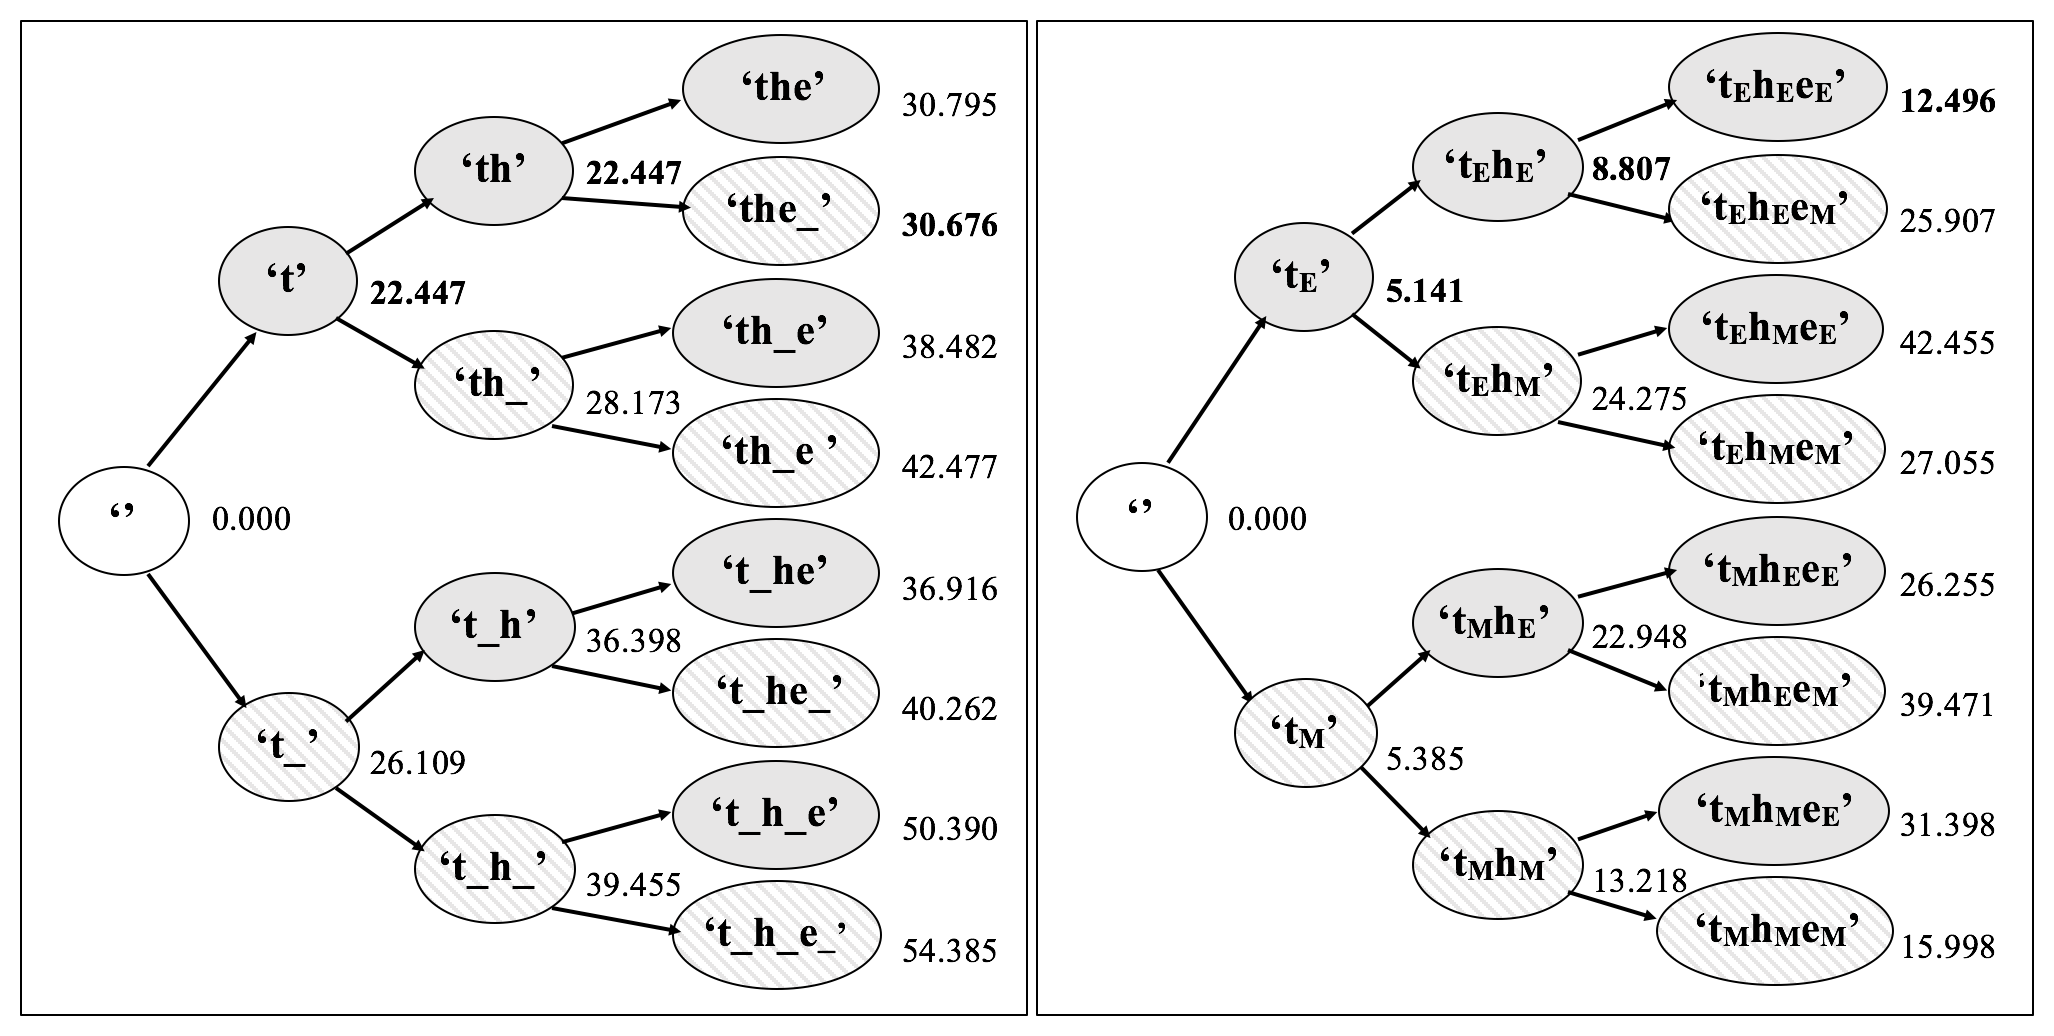
\includegraphics[height=3.6in,width=5.1in]{search-trees}
\caption{Search trees for the sample text `{\it the}' for the word segmentation problem (on the left) and for the language segmentation problem (on the right).}

\label{figure:search-trees}
\end{figure}

The search tree for the language segmentation problem (using the tool {\bf markup}) is shown in the right box. The tree in this example also has a branching of two as only two transformations are being used here for the languages being segmented---English and M$\bar{\textrm{a}}$ori. Hence the search process is analogous to the word segmentation problem---instead of a space being added or not, the transformation simply decides to code the symbol being processed using the English model for the gray nodes or using the M$\bar{\textrm{a}}$ori model for the hashed nodes. The subscripts shown in the transformed sequences within each node indicate which model was used to code each
symbol---the subscript `E' if the English model was used and the subscript `M' if the M$\bar{\textrm{a}}$ori model was used instead. If a
symbol switches coding from one model to the other, then the sentinel symbol is encoded which will incurr a significant cost as it will have to back off to the null context as a result.

Shown to the right  of each node in both trees is the compression codelength for the transformed sequence as calculated by the toolkit (based on a static order 5 PPMD model trained on the Brown corpus for the left box, and static order 5 PPMD models trained on the English and M$\bar{\textrm{a}}$ori bibles for the right box). The smallest codelength for each level of the tree is shown in bold font. Note that these trees show the complete search tree as if a breadth-first search was being applied.  In reality, many of the nodes in the full trees would be pruned away depending on the search algorithm being applied based on these
compression codelength values. (For example, for the Viterbi algorithm, all nodes at the same level of the tree with the same conditioning context for the maximum order of the model would be pruned except for the one with the lowest codelength).

\begin{table}
{\tabcolsep 0.50mm
\begin{tabular}{lcccc} \hline
{\bf Algorithm} & {\bf Editdistance} & {\bf Edistance} & {\bf Average Time} & {\bf Number of} \\
& & {\bf Accuracy (\%)} & {\bf (seconds)} & {\bf nodes} \\ \hline
Viterbi                  & 493 & 99.17 &   2.657 & 2391680 \\
Stack (size = 5)   & 787 & 98.69 &   1.315 & 2338160 \\
Stack (size = 10) & 620 & 98.96 &   2.339 & 2345280 \\
Stack (size = 20) & 568 & 99.05 &   4.369 & 2348080 \\
Stack (size = 50) & 533 & 99.11 & 10.386~\, & 2443560 \\
\hline
\end{tabular}
\caption{Results from using various search algorithms for the {\bf segment} tool to segment the first 10,000 words of the unsegmented LOB corpus using a static order 5 PPMD model trained on the Brown corpus using the {\bf train} tool.}
\label{table.search}
}
\end{table}

Table~\ref{table.search} lists some experimental results for the two search algorithms implemented by the toolkit---the Viterbi algorithm and the stack algorithm. In this case, the {\bf segment} tool was used to segment the first 10,000 words of the unsegmented LOB corpus using a static order 5 PPMD model trained on the Brown corpus using the {\bf train} tool. Shown in the table are the following: a description of the algorithm used (including the size of the stack if the stack algorithm was used); the Levenshtein editdistance ($e$) between the correct LOB source text and the output produced by the tool (where the cost of a deletion and an insertion was counted as 1, and of a substitution as 2); the editdistance accuracy as a percentage calculated as $100 - 100 \times e / N$ where $N$ was the size of the source text; the average time in seconds to complete the segmentation task for 10 runs on the Macbook Pro; and the number of nodes that were
generated in the search tree as a measure of the memory used. The results show that the Viterbi algorithm produces the least number of errors, and the number of errors reduces with a larger stack size for the stack algorithm as expected. However, the time and memory results show that a smaller stack size runs more quickly (twice as fast when the stack size is only 5) and uses less memory but at a cost in reduced accuracy. Therefore, if speed and/or memory is a concern (when processing many texts or texts that are much larger in size), then accuracy can be traded for improved speed and memory by choosing the stack algorithm. These results mirror those published for the
Chinese word segmentation problem using an earlier version of the toolkit~\cite{tea00a} and confirm that the latest version produces
similar behaviour.

\section{Experimental results obtained using the toolkit}
\label{section.results}

This section provides a summary in Table~\ref{table.results} of a selection of published experimental results that were produced using the applications in the toolkit. The table lists the publication, the toolkit tools that were used to obtain the experimental results, and the specific application area, such as emotion recognition in text, gender and authorship categorisation and so on. The purpose is to show the wide variety of application areas that the toolkit can be applied to and also to provide supporting evidence of the effectiveness of the algorithms detailed in Section~\ref{section.samples}. For example, the classification results achieved using the {\bf classify} tool consistently outperform well-known feature-based approaches such as SVM and Na\"{\i}ve Bayes in many application areas. The reader should refer to the publications directly for full details concerning the experimental methodology involved and the results obtained.

\begin{table}
{\tabcolsep 0.55mm
\begin{tabular}{lp{2.7cm}p{4.7cm}} \hline
{\bf Reference} & {\bf Tools used} & {\bf Application area} \\ \hline
& \\

Alamri \& Teahan~\shortcite{ala17} & {\bf classify}, {\bf train} & Classifying dyslexic text \\
Al-Kazaz {\em et al.}~\shortcite{alk16} & {\bf codelength}, {\bf train} & Cryptanalysis of transposition cipehers \\
Alkahtani {\em et al.}~\shortcite{slt15} & {\bf align}, {\bf train} & English-Arabic bilingual sentence alignment \\
Alkhazi \& Teahan~\shortcite{alk17} & {\bf classify}, {\bf markup}, {\bf train} & Classifying and segmenting Arabic text \\
Al-Mahdawi \& Teahan~\shortcite{alm17} & {\bf classify}, {\bf train} & Emotion recognition in text \\
Altamimi \& Teahan~\shortcite{alt17} & {\bf classify}, {\bf train} & Gender and authorship categorisation of Arabic text \\
Liu \& Teahan~\shortcite{liu14} & {\bf align}, {\bf train} & English-Chinese bilingual sentence alignment \\
Mahoui {\em et al.}~\shortcite{mah08} & {\bf markup}, {\bf train} & Identification of gene function in biological publications \\
Teahan \& Aljehane~\shortcite{alj17} & {\bf encode}, {\bf decode} & Grammar-based compression \\
Teahan \& Alhawiti~\shortcite{alh15} & {\bf encode}, {\bf decode} & Compression of Arabic text \\
\hline
\end{tabular}
\caption{A summary of selected experimental results produced using the toolkit.}

\label{table.results}
}
\end{table}

\section{Related work}

Many different toolkits, suites, architectures, frameworks, libraries,  APIs and/or development environments have been produced over the years for natural language processing purposes and more specifically for statistical natural language processing. The use of these terms to describe the functionality and nature of the various NLP systems and approaches have often been inconsistent in the literature. For example,  Cunningham~\shortcite{cun02} stated for the GATE system---a general `architecture' for text engineering---that it ``{\em is generally referred to as an `architecture', when, if we were a little more pedantic, it would be called a framework, architecture and development environment}''. The meaning of the term `framework' in software engineering has also evolved over the years---its more specific meaning in recent years requires that a framework has the key characteristic of `inversion of control' where a framework must handle the flow of control of the application. This characteristic is not appropriate for the design used for the Tawa toolkit's libraries which do not handle the flow of control in many of its applications (except for when $Transform$ objects are used). The meaning of the term `architecture' is clearer in the literature---it involves the abstract
design concepts and structures behind an application. For these reasons for the work described in this paper, the well accepted terms toolkit, libraries and architecture have been used to describe the system, and its design and implementation.

\begin{table}
{\tabcolsep 0.55mm
\begin{tabular}{llp{4.5cm}l} \hline
{\bf System} & {\bf Reference} & {\bf Type of system} & {\bf Language(s)} \\ \hline
CoreNLP & \cite{man14} & suite of tools & Java \\
FreeLing & \cite{car04} & library & C++ \\ 
GATE & \cite{cun02} & architecture, suite of tools  & Java \\
LingPipe & \cite{car06} & toolkit, API & Java \\ 
MALLET & \cite{mcc02} & toolkit, API & Java \\ 
NLTK & \cite{bir06} & library & Python \\ 
OpenNLP & \cite{bal05} & library & Java  \\
%SpaCy & \cite{hon15} & library & Python, Cython  \\
Tawa & (This paper) & toolkit, libraries & C \\
UIMA & \cite{fer04} & architecture, middleware & Java, C++ \\
\hline
\end{tabular}
\caption{Some systems for NLP and their details.}

\label{table.systems}
}
\end{table}

Table~\ref{table.systems} lists a selection of systems that have been developed for NLP. The table lists the name of the system, a reference, the type of system described using terms used by the developers of the system and the language(s) in which the system has been developed. The table illustrates that there have been many systems developed to date in a number of different programming languages with Java predominating. The preferred type of system is a toolkit and/or an external library being available. These systems in general provide a suite of tools for various applications, such as tokenisation, classification, POS tagging, named entity recognition and parsing being the ones provided the most.

A number of further freely available systems that have been developed by the NLP research community are based on a range of underlying architectures including those listed in Table~\ref{table.systems}. For example, DKPro and ClearTK  are two examples that use the UIMA framework architecture for analysing unstructured information. Alternatively, some of the systems are primarily designed around a core external library or libraries that can be called from an application. Often these systems are not described as having an underlying architecture (for example, FreeLing, NLTK and OpenNLP in the table). The two main approaches all of these systems use for text processing involve a rule-based approach (either manually designed or automatically generated) and statistical. These systems also
predominantly process natural language text in a word-based manner.

What distinguishes the Tawa toolkit from most of these systems is threefold: firstly, the toolkit is character-based; secondly, 
the design of the applications is based around an integrated compression-based architecture; and thirdly, none of the toolkits in the table (apart from Tawa itself), provide explicit support for compression-based applications.
Tawa is also written from the ground up with carefully memory-managed C code for each object type and therefore is designed to be memory efficient and fast.

Like the Tawa system, the LingPipe system also uses character language models but uses the noisy channel model approach for various applications. Using a character or symbol-based approach means that methods used for solving the tasks required for
applications can be quite different to the traditional word-based approach. For example, the Tawa toolkit for classification avoids the need for explicit word-based feature extraction and simply processes all the characters in the text being classified.

The application of compression-based models to NLP has had a long history and one of the main purposes of the Tawa toolkit is to make these models more easily available for developers to use. In many cases, the applications implemented using these models have produced state-of-the-art results. For example, PPM character based language models have been applied successfully to many applications in natural language processing~\cite{tea98} such as language identification and cryptography~\cite{irv97} including various applications for automatically correcting words in texts such as OCR and word segmentation~\cite{tea98a,tea00} (also see Table~\ref{table.results} for a further selection of results). 

Text mining and named entity extraction in Tawa can also be performed using character-based language models using an approach similar to that used by Mahoui {\em et al.}~\shortcite{mah08} to identify gene function. Bratko~\shortcite{bra12} have also used data compression models for text mining, specifically for spam filtering. Witten {\it et al}.~\shortcite{wit99a,wit99b} have shown how text compression can be used as a key technology for text mining. Here, character-based language modelling techniques based on PPM to detect sub-languages of text instead of explicit programming are used to extract meaningful low-level information about the location of semantic tokens such as names, email addresses, locations, URLs and dates. In this approach, the training data for the model of the target text contains text that is already marked up in some  manner. A correction process is then performed to recover the most probable target text (with special markup symbols inserted) from the  unmarked-up source text. Yeates {\em et al.}~\shortcite{yea01} show how many text mining applications can be recast as `tag insertion' problems such as word segmentation and identifying acronyms in text~\cite{yea00} where tags are re-insert back into a sequence to reveal the meta-data implicit in it. Teahan \& Harper~\cite{tea01} describe a competitive text compression scheme which also adopts this tag insertion model. The scheme works by switching between different PPM models, both static and dynamic (i.e. that adapt to the text as it is being encoded). Tags are inserted to indicate where the encoder has switched between models. Tag insertion problems, however, are just part of a much broader class of applications encompassed by the noiseless channel model and therefore possible using the Tawa toolkit. The toolkit diverges substantially from the tag insertion model of Yeates {\em et al}.~\shortcite{yea01} (by allowing regular expressions and functions in the specification of both the matching source sequence and corrected target sequence) and arguably also the noisy channel model approach (for example, by making it easier to combine models using hybrid encoding methods or by using preprocessing techniques to modify alphabets).

\section{Conclusion and future work}

A novel toolkit for text processing\footnote{The toolkit can also process general text not just natural language text and has been applied successfully to the processing of the following types of textual data, for example: compression of source code, bibliographic references, Unix terminal session transcriptions and executable program files; analysis of complex system output including cellular automata and flocking simulations; and even the textual transcription of bird song.} and natural language processing has been described. The underlying architecture is based on using an encoding approach: that of characterising applications as a problem of searching for the best encoding of the target text given the source text. The toolkit implements various types of  compression models, as well as several search algorithms, and various NLP applications. These compression-based models process the text sequentially and base their predictions of the upcoming character on a fixed length finite context of preceding characters. Experimental results have shown that these models are competitive against alternative word-based approaches adopted by most other NLP systems.

Like the noisy channel model, the `noiseless channel model' architecture adopted by the toolkit models the text processing as sending a message down a communication channel. This design of the toolkit adheres to two main principles---the communication process must be both {\it lossless} and {\it reversible}. All information in the message is communicated without loss, and therefore any transformation of the source text to the target text is done in such a way that the source text is recoverable. Unlike the noisy channel model where the source text is unknown when it is decoded, the source text in the approach adopted by the toolkit is known when it is encoded, therefore providing an opportunity
that a more effective encoding can be found more efficiently.

Future work will involve the application of this new model to further text processing problems that have not yet been investigated fully
such as POS tagging, named entity recognition, OCR and machine translation. Also other approaches similar to the joint source-channel model approach of Haizhou {\em et al.}~\shortcite{hai04} for machine transliteration will also be investigated where the best encoding of both the source and target messages are generated simultaneously as this can be easily accommodated using the toolkit's architecture.


\begin{thebibliography}{}

     \bibitem[\protect\citename{Abel and Teahan } 2005]{at05}
     Abel, J. and Teahan, W. (2005)
     ``Universal text preprocessing for data compression''. {\em IEEE Transactions on Computers}, 54(5), pp. 497--507.

     \bibitem[\protect\citename{Alamri and Teahan }2017]{ala17}
     Alamri, M. and Teahan, W.J. (2017)
     ``Distinguishing Dyslexic Text from Regular Text using PPM for the possible publication''. Submitted to {\em International Journal of
     Computational Linguistics (IJCL)}, Volume 8, Issue 1.

     \bibitem[\protect\citename{Alhawiti }2014]{alh14}
     Alhawiti, K.M. (2014) {\em Adaptive models of Arabic text}. Ph.D. thesis,
     Bangor University, Wales.

    \bibitem[\protect\citename{Alkahtani {\it et al.}\ }2015]{slt15}
    Alkahtani S., Liu, W. and Teahan, W.J. (2015)
    ``A new hybrid metric for verifying parallel corpora of Arabic-English'' in
    {\em Proceedings of the Fifth International Conference on Computer Science, Engineering and Applications (CCSEA-2015)}'',
    Dubai, UAE.

    \bibitem[\protect\citename{Al-Kazaz  {\it et al.}\ }2016]{alk16}
    Al-Kazaz, N.R., Irvine, S.A. and Teahan, W.J. (2016)
    ``An Automatic Cryptanalysis of Transposition Ciphers Using Compression'' in
    {\em International Conference on Cryptology and Network Security}, pp. 36--52. Springer International Publishing.

    \bibitem[\protect\citename{Alkhazi and Teahan }2017]{alk17}
    Alkhazi, I.S. and Teahan, W.J. (2017)
    ``Classifying and Segmenting Classical and Modern Standard Arabic using Minimum Cross-Entropy''.
    {\em International Journal of Advanced Computer Science and Applications}, 8(4), pp. 421--430.

    \bibitem[\protect\citename{Alkhazi {\it et al.}\ }2017]{alk17a}
    Alkhazi, I.S., Alghamdi, M.A. and Teahan, W.J. (2017)
    ``Tag based models for Arabic text compression'' in {\em Proceedings of the Intelligent Systems Conference}, 7-8 September,
    London, UK.

    \bibitem[\protect\citename{Al-Mahdawi and Teahan }2017]{alm17}
    Al-Mahdawi, A. and Teahan, W.J. (2017)
    ``Emotion Recognition in Text Using PPM'' in
    {\em Proceedings of the AI-2017: The Thirty-seventh SGAI International Conference}. Cambridge, UK.

    \bibitem[\protect\citename{Anderson and Moran }1984]{and84}
    Anderson, J.B. and Mohan, S. (1984)
    ``Sequential coding algorithms: A survey and cost analysis.''
    {\em IEEE Transactions on Communications}, {\bf 32}(2), pp. 169--176.

    \bibitem[\protect\citename{Altamimi and Teahan }2017]{alt17}
    Altamimi, M. and Teahan, W.J. (2017)
    ``Gender and authorship categorisation of Arabic text from Twitter using PPM''.
    {\em International Journal of Computer Science and Information Technology (IJCSIT)}. 

    \bibitem[\protect\citename{Baldridge }2005]{bal05}
    Baldridge, J. (2005) {\em The opennlp project}. URL: \url{http://opennlp.apache.org/index.html}, (accessed 18 October, 2017).

    \bibitem[\protect\citename{Bell {\it et al.}\ }1990]{bcw90}
    Bell, T.C., Cleary, J.G. and Witten, I.H. (1990) {\em Text compression}. Prentice-Hall, Inc..

    \bibitem[\protect\citename{Bratko }2012]{bra12}
    Bratko, A. {\em Text mining using data compression models}. Doctoral thesis. University of Ljubljana.

    \bibitem[\protect\citename{Bird }2006]{bir06}
    Bird, S. (2006)
    ``NLTK: the natural language toolkit'' in
    {\em Proceedings of the COLING/ACL on Interactive presentation sessions},  pp. 69--72. Association for Computational Linguistics.

    \bibitem[\protect\citename{Burrows and Wheeler }1994]{bw94}
    Burrows, M. and Wheeler, D.J. (1994) ``A block-sorting lossless data compression algorithm''.
    Technical report 124, 1994, Palo Alto, CA. Digital Equipment Corporation.

    \bibitem[\protect\citename{Carpenter }2006]{car06}
    Carpenter, B. (2006)
    ``Character language models for Chinese word segmentation and named entity recognition'' in
    {\em Proceedings of the Fifth SIGHAN Workshop on Chinese Language Processing}, pp. 169--172.

    \bibitem[\protect\citename{Carreras {\it et al.} }2004]{car04}
    Carreras, X., Chao, I., Padr\'{o}, L. and Padr\'{o}, M. (2004)
    ``FreeLing: An Open-Source Suite of Language Analyzers'' in
    {\em Proceedings of the 4th International Conference on Language Resources and Evaluation (LREC'04)}.

    \bibitem[\protect\citename{Cleary and Witten }1984]{cle84}
    Cleary, J.G. and Witten, I.H. (1984)
    ``Data compression using adaptive coding and partial string matching.''
    {\em IEEE Transactions on Communications}, {\bf 32}(4), pp. 396--402.

    \bibitem[\protect\citename{Cleary and Teahan }1997]{cle97}
    Cleary, J.G. \& Teahan, W.J. (1997)
    ``Unbounded length contexts for PPM.''
    {\em Computer Journal}, {\bf 40}(2/3), pp. 67--75.

    \bibitem[\protect\citename{Cunningham }2002]{cun02}
    Cunningham, H. (2002)
    ``GATE, a general architecture for text engineering''. {\em Computers and the Humanities}, {\bf 36}(2), pp. 223--254.

    \bibitem[\protect\citename{Ferrucci and Lally }2004]{fer04}
    Ferrucci, D. and Lally, A. (2004)
    ``UIMA: an architectural approach to unstructured information processing in the corporate research environment''.
    {\em Natural Language Engineering}, 10(3-4), pp. 327--348.

    \bibitem[\protect\citename{Francis and Ku\u{c}era }1979]{fra79}
    Francis, W.N. and Ku\u{c}era, H. (1979) {\em Brown corpus manual}. Brown University.

    \bibitem[\protect\citename{Haizou {\it et al.} }2004]{hai04}
    Haizhou, L., Min, Z. and Jian, S. (2004)
    ``A joint source-channel model for machine transliteration'' in
    {\em Proceedings of the 42nd Annual Meeting on association for Computational Linguistics}. Association for Computational Linguistics.

     \bibitem[\protect\citename{Hockenmaier and Brew }1998]{hoc98}
     Hockenmaier, J. \& Brew, C. 1998.
     ``Error-driven learning of Chinese word segmentation'' in
     {\em 12th Pacific Conference on Language and Information}, edited by
     Guo, J., Lua, K.T. \& Xu, J., Singapore, Chinese and Oriental Languages
     Processing Society, pp. 218--229.

%    \bibitem[\protect\citename{Honnibal and Montani }2015]{hon15}
%    Honnibal, M. and Montani, I. (2015)
%    {\em spaCy, an open-source library for industrial-strength NLP}.
%    URL: \url{https://spacy.io} (accessed 18 October, 2017).

    \bibitem[\protect\citename{Irvine }1997]{irv97}
    Irvine, S.A. (1997)
    {\em Compression and Cryptology}. D.Phil. thesis,
    University of Waikato, N.Z.

    \bibitem[\protect\citename{Jelinek }1969]{jel69}
    Jelinek, F. (1969)
    ``Fast sequential decoding algorithm using a stack''.
    {\em IBM journal of research and development},13(6), pp. 675--685.

    \bibitem[\protect\citename{Johansson {\it et al.} }1986]{joh86}
    Johansson, S., Atwell, E., Garside, R. and Leech, G. (1986)
    {\em The tagged LOB Corpus}. Norwegian Computing Centre for the Humanities, Bergen.

    \bibitem[\protect\citename{Kernighan {\it et al.} }1990]{ker90}
    Kernighan, M.D., Church, K.W. and Gale, W.A. (1990)
    ``A spelling correction program based on a noisy channel model'' in
    {\em Proceedings of the 13th conference on Computational linguistics}, Volume 2, pp. 205--210).
    Association for Computational Linguistics.

     \bibitem[\protect\citename{Khmelev and Teahan }2003]{kt03}
     Khmelev, D.V. and Teahan, W.J. (2003)
     ``A repetition based measure for verification of text collections and for text categorization'' In
     {\em Proceedings of the 26th annual international ACM SIGIR conference on Research and development in Information Retrieval},
     pp. 104--110). ACM.

    \bibitem[\protect\citename{Knight }1999]{kni99}
    Knight, K. (1999) ``Mining on-line text'' in
    {\em Communications of the ACM}, {\bf 42}(11), pp. 58--61.

    \bibitem[\protect\citename{Liu and Teahan  }2014]{liu14}
    Liu, W. and Teahan, W.J. (2014)
    ``PPM Compression-based Method for English-Chinese Bilingual Sentence Alignment''. {\em Lecture Notes in Computer Science},
    Volume 8791, {\em Statistical Language and Speech Processing Second International Conference, SLSP 2014}, Grenoble, France,
    October 14-16, 2014. Editors: Laurent Besacier, Adrian-Horia Dediu, Carlos Mart�n-Vide.

    \bibitem[\protect\citename{Mahoui {\it et al.}\ }2008]{mah08}
    Mahoui, M., Teahan, W.J., Thirumalaiswamy Sekhar, A.K. and Chilukuri, S. (2008)
    ``Identification of gene function using prediction by partial matching ({PPM}) language models'' in
    {\em Proceedings of the 17th ACM Conference on Information and Knowledge Management}, pp. 779--786. ACM.

    \bibitem[\protect\citename{Manning {\it et al.}\ }2014]{man14}
    Manning, C.D., Surdeanu, M., Bauer, J., Finkel, J., Bethard, S.J. and McClosky, D. (2014)
    ``The Stanford CoreNLP Natural Language Processing Toolkit'' in
    {\em Proceedings of the 52nd Annual Meeting of the Association for Computational Linguistics: System Demonstrations}, pp. 55--60.

    \bibitem[\protect\citename{McCallum }2002]{mcc02}
    McCallum, A.K. (2002) ``MALLET: A Machine Learning for Language Toolkit.''
    URL: \url{http://mallet.cs.umass.edu.}, (accessed 17 October, 2017).

    \bibitem[\protect\citename{Moffat }1990]{mof90}
    Moffat, A. (1990)
    ``Implementing the PPM data compression scheme.''
    {\em IEEE Transactions on Communications}, {\bf 38}(11), pp. 1917--1921.

    \bibitem[\protect\citename{Rissanen and Langdon  }1979]{rl79}
    Rissanen, J. and Langdon, G.G. (1979) ``Arithmetic coding''.
    {\em IBM Journal of research and development}, 23(2), pp. 149--162.

    \bibitem[\protect\citename{Rissanen and Langdon  }1981]{rl81}
    Rissanen, J. and Langdon, G.G. (1981)
    ``Universal modeling and coding''. {\em IEEE Transactions on Information Theory}, 27(1), pp. 12--23.

     \bibitem[\protect\citename{Shannon }1948]{sha48}
     Shannon, C.E. (1948) ``A mathematical theory of communication.''
    {\em Bell System Technical Journal}, {\bf 27}, pp. 379--423, 623--656.

    \bibitem[\protect\citename{Sproat and Emerson  }2003]{spr03}
    Sproat, R. and Emerson, T. (2003).
    ``The first international Chinese word segmentation bakeoff'' in
    {\em Proceedings of the second SIGHAN workshop on Chinese language processing}. Volume 17, pp. 133--143. ACL.

     \bibitem[\protect\citename{Teahan }1998]{tea98}
     Teahan, W.J. (1998) {\em Modelling English text}. D.Phil. thesis,
     University of Waikato, N.Z.

     \bibitem[\protect\citename{Teahan }2000]{tea00a}
     Teahan, W.J. (2000)
     ``Text classification and segmentation using minimum cross-entropy'' in
     {\em Content-Based Multimedia Information Access}, Volume 2, pp. 943--961. Le Centre de Hautes Etudes Internationales
     D'Informatique Dcoumentaire.

    \bibitem[\protect\citename{Teahan and Aljehane  }2017]{alj17}
    Teahan, W.J. and Aljehane, N.O. (2017)
    ``Grammar based pre-processing for PPM''.
    {\em International Journal of Computer Science and Information Security},�9(1).

    \bibitem[\protect\citename{Teahan and Alhawiti  }2015]{alh15}
    Teahan, W. J. and Alhawiti, K. M. (2015)
    ``Preprocessing for PPM: Compressing UTF-8 Encoded Natural Language Text''.
    {\em International Journal of Computer Science and Information Technology (IJCSIT)}, Vol. 7, No. 2, April.

     \bibitem[\protect\citename{Teahan {\it et al.}\ }1998]{tea98a}
    Teahan, W.J., Inglis, S., Cleary, J.G. \& Holmes, G. (1998)
    ``Correcting English text using PPM models'' in
    {\em Proceedings DCC'98}, edited by Storer, J.A. \& Cohn, M.,
    IEEE Computer Society Press.

     \bibitem[\protect\citename{Teahan {\it et al.}\ }2000]{tea00}
    Teahan, W.J., Wen, Y.Y., McNabb, R. \& Witten, I.H. (2000)
    ``Using compression models to segment Chinese text''. {\em Computational Linguistics}, 26(3), pp. 375--393.

     \bibitem[\protect\citename{Teahan and Harper }2001]{tea01}
     Teahan, W.J. and Harper, D.J. (2001)
     ``Combining PPM models using a text mining approach'' in
     {\em Proceedings of the Data Compression Conference 2001}, pp. 153--162. IEEE.

     \bibitem[\protect\citename{Teahan and Harper }2003]{tea03}
     Teahan, W.J. and Harper, D.J. (2003)
     ``Using compression-based language models for text categorization'' in
     {\em Language modeling for information retrieval}, 141-165. Springer Netherlands.

    \bibitem[\protect\citename{Witten {\it et al.}\ }1987]{wit87}
    Witten, I.H., Neal, R.M. and Cleary, J.G. (1987)
    ``Arithmetic coding for data compression''. {\em Communications of the ACM}, 30(6), pp. 520--540. Vancouver.	

     \bibitem[\protect\citename{Witten and McNab }1997]{wit97}
     Witten, I.H. and McNab, R. (1997)
     ``The New Zealand Digital Library: Collections and Experience''. {\em The Electronic Library}. 15(6), pp. 495--504.

    \bibitem[\protect\citename{Witten {\it et al.}\ }1999a]{wit99a}
    Witten, I.H., Bray, Z., Mahoui, M. \& Teahan, W.J. (1999a)
    ``Text mining: A new frontier for lossless compression'' in
    {\em Proceedings DCC'99}, edited by Storer, J.A. \& Cohn, M.,
    IEEE Computer Society Press.

    \bibitem[\protect\citename{Witten {\it et al.}\ }1999b]{wit99b}
    Witten, I.H., Bray, Z., Mahoui, M. \& Teahan, W.J. (1999b)
    ``Using language models for generic entity extraction'' in
    {\em ICML-99 Worskhop: Machine learning in text data analysis}.

    \bibitem[\protect\citename{Viterbi }1967]{vit67}
    Viterbi, A.J. (1967) ``Error bounds for convolutional codes and an
    asymptotically optimal decoding algorithm,'' {\em IEEE Transactions on
    Information Theory}, {\bf 13}, pp. 260--269.

     \bibitem[\protect\citename{Volf and Willems }1998]{vol98}
     Volf, P.A. and Willems, F.M. (1998)
     ``Switching between two universal source coding algorithms'' in
     {\em Proceedings of the Data Compression Conference, 1998}, pp. 491--500. IEEE.

    \bibitem[\protect\citename{Yeates {\it et al.}\ }2000]{yea00}
    Yeates, S., Bainbridge, D. and Witten, I.H. (2000)
    ``Using compression to identify acronyms in text''. {\em arXiv preprint cs/0007003}.
    
    \bibitem[\protect\citename{Yeates {\it et al.}\ }2001]{yea01}
    Yeates, S., Witten, I.H. and Bainbridge, D. (2001)
    ``Tag insertion complexity'' in {\em Proceedings of the Data Compression Conference 2001}, pp. 243--252. IEEE.

     \bibitem[\protect\citename{Ziv and Lempel }1977]{zl77}
     Ziv, J. and Lempel, A. (1977)
     ``A universal algorithm for sequential data compression''.
     {\em IEEE Transactions on Information Theory}, 23(3), pp. 337--343.

     \bibitem[\protect\citename{Ziv and Lempel }1978]{zl78}
     Ziv, J. and Lempel, A. (1978)
     ``Compression of individual sequences via variable-rate coding''.
     {\em IEEE transactions on Information Theory}, 24(5), pp. 530--536.

\end{thebibliography}

\end{document}
